% Draft 2 of 2026-10-07 (evening). Sources: lemma/PROOF_C2/{MAIN,A1_REDUCTION,A2_BRIDGE,A3_LEMMAS,B_LATTICES}.md,
% lemma/upstream/{LATTICE_143,AUDIT_ENGINE_RULES,AUDIT_REDUCTION}.md. Appendix A is generated (table156.tex, lab session).
%
% OPEN POINTS, to be closed before circulation (search for "TODO"):
%  1. (closed 07/10, author's instruction) Sole author: Dilan Djematene; AI assistance in the Acknowledgements, without
%     naming a model. The correspondence address he wants printed is still to be added. All the Conway repositories of
%     the account are private since 07/10. The links are printed (his instruction: the papers are not published now, he
%     opens the repositories when they are); the repositories must be public before the paper is circulated.
%  2. (closed 07/10, 20:31 UTC) Lattice 044: second run finished and accepted by the lab's check; Section 8.5 updated.
%  3. (closed 07/10) Packing numbers of Table 1: reproduced by a second program (Codex, q/codex_independent_packing.py) and,
%     for test (a), by a third (lab); Section 9 says so.
%  4. Bibliography (07/10, 20:45 UTC: the published paper [CW] was read directly, pp. 379-380 and its reference list;
%     its Introduction gives the history (Biggs, Guy, Conway's prize), the family k = u^2+u+2, "[MM, Theorem 2.7]: |G|
%     divides 2.3^3.7.11", "[Mak, Corollary 2.4]: an involution implies |G| divides 42 (or 6)", "Behbahani-Lam: any
%     automorphism of prime order has order 2 or 3", "Crnkovic-Maksimovic: no group of order 6 or 9"; so those
%     attributions now rest on [CW]'s own summary. Behbahani-Lam and the thesis themselves are still not opened.)
%     Earlier note: the statements attributed to [MM], [Mak], [B09], [BL] in the Introduction follow the literature section
%     of the author's manuscript on order 3 (with its theorem numbers) and the abstract of [CW]; the papers themselves were
%     not opened for this text. [CW], [CM], [CS90], [Bor] were checked on the publishers' pages on 07/10. The section
%     number of the oddity formula in [SPLAG] is to be added. [D3] is in a private repository: give its public location.
%  5. T20: reserve G2 of the referee (wording of the verifier's contract) in the supplement.
%  6. One frozen referee pass on this text. New with respect to the refereed Part A: property (R8) is stated separately
%     (it is A.5); Lemma 6.2 (the u_o generate N; connectivity) and Lemma 6.6 (twins) are written out; Proposition 8.1.
\documentclass[11pt]{amsart}
\usepackage[utf8]{inputenc}
\usepackage[T1]{fontenc}
\usepackage{lmodern}
\usepackage{amsmath,amssymb,amsthm}
\usepackage[margin=1.15in]{geometry}
\usepackage{booktabs,longtable}
\usepackage{enumitem}
\usepackage[hidelinks]{hyperref}
\usepackage{tikz}
\usetikzlibrary{arrows.meta,positioning}

\newtheorem{theorem}{Theorem}[section]
\newtheorem{proposition}[theorem]{Proposition}
\newtheorem{lemma}[theorem]{Lemma}
\newtheorem{corollary}[theorem]{Corollary}
\theoremstyle{definition}
\newtheorem{definition}[theorem]{Definition}
\theoremstyle{remark}
\newtheorem{remark}[theorem]{Remark}

\newcommand{\Z}{\mathbb{Z}}
\newcommand{\R}{\mathbb{R}}
\newcommand{\F}{\mathbb{F}}
\newcommand{\G}{\Gamma}
\newcommand{\s}{\sigma}
\newcommand{\rk}{\operatorname{rank}}
\newcommand{\Pl}{\Pi}
\newcommand{\repo}{\texttt{github.com/amazing-source/conway99-c2-aws}}

\title[No involution on a strongly regular graph $(99,14,1,2)$]{A strongly regular graph with parameters $(99,14,1,2)$\\ has no automorphism of order two}
\author{Dilan Djematene}
\date{Draft of 7 October 2026}
\subjclass[2020]{Primary 05E30; Secondary 05C25, 11H06, 11H55, 68V05}
\keywords{Strongly regular graph, Conway's 99-graph problem, automorphism group, involution, unimodular lattice, tight
frame, computer-assisted proof}

\begin{document}

\begin{abstract}
Conway's 99-graph problem asks whether there is a strongly regular graph with parameters $(99,14,1,2)$. We prove that such a
graph has no automorphism of order $2$. The first half of the proof is done by hand: from the definition of the graph, an
involution produces a tight frame of $51$ vectors inside an odd unimodular lattice of rank $24$ without vectors of norm $1$,
hence inside one of the $156$ lattices of Borcherds' classification. The second half is computer-assisted and shows that none
of the $156$ lattices contains such a frame. Twenty lattices are excluded by short arguments on the lattice itself. For the
$136$ others, the pairs of vectors of norm $7$ that could be the two normals of the frame are enumerated up to symmetry and
excluded one by one: by a short vector whose existence contradicts one of three nonexistence lemmas for integer eigenfunctions
of small norm, with an exact certificate for each pair, by transfer to another lattice of the list, or by an exhaustive search for the frame. We state which steps were
verified by independent programs and which rest on a single audited program. This draft records the state of that computation: one validation, the recertification of a part of the transfers
(Section~\ref{sec:verif}), remains to be completed. The programs, run summaries and certificates are kept in the
accompanying repository, private at the time of writing. Together with the known exclusions of the odd prime orders, the theorem implies that a strongly regular graph with
parameters $(99,14,1,2)$, if it exists, has no nontrivial automorphism; that consequence and its dependencies are the
subject of a separate note.
\end{abstract}

\maketitle

\section{Introduction}

A strongly regular graph with parameters $(v,k,\lambda,\mu)$ is a $k$-regular graph on $v$ vertices in which two adjacent
vertices have exactly $\lambda$ common neighbours and two distinct non-adjacent vertices exactly $\mu$. Whether a strongly
regular graph with parameters $(99,14,1,2)$ exists is one of Conway's five problems \cite{Conway}. Its adjacency matrix would
have the eigenvalues $14$, $3$ and $-4$ with multiplicities $1$, $54$ and $44$, and the standard feasibility conditions do not
exclude it. A graph with these parameters is now usually called a \emph{Conway $99$-graph}; the introduction of \cite{CW}
recounts how the question arose, half a century ago, and how it came to carry a prize. Among the parameter sets $(v,k,1,2)$,
Makhnev and Minakova \cite{MM} showed that only five values of $k$ are possible, namely $k=u^2+u+2$ for $u=1,3,4,10,31$. The
first and the third are realised, by the $3\times3$ rook's graph and by a graph on $243$ vertices built from the ternary
Golay code; our case is $u=3$, and for it, as for $u=10$ and $u=31$, no graph is known. An early structural study of the graph on $99$ vertices is due to Wilbrink \cite{W84}. For strongly regular graphs in general we refer to \cite{BvM,GR}.

Most of what is known concerns the automorphism group $G$ of such a graph $\G$. Makhnev and Minakova \cite{MM} proved by
character theory that $|G|$ divides $2\cdot3^3\cdot7\cdot11$; if $|G|$ is even it divides $42$ \cite{MM,Mak}. Behbahani and
Lam \cite{B09,BL} showed, by a computer enumeration of orbit matrices, that the only primes that can divide $|G|$ are $2$
and $3$, and that an automorphism of order $3$ has no fixed point. Crnkovi\'c and Maksimovi\'c \cite[Theorems~7.2 and~7.3]{CM} excluded, also by computer, groups of automorphisms of order $6$ and $9$. Cesarz and Woldar \cite[Corollaries~3.13 and~4.15]{CW} proved without a computer that
$G\cong\Z_7$ if $7$ divides $|G|$, and consequently that $|G|$ divides $6$ if it is even; this does not exclude an
automorphism of order $7$, which remained open without a computer. Together these results left $|G|\in\{1,2,3\}$. Two
manuscripts of the present project treat odd orders: order $3$ is excluded in \cite{D3} by linear algebra over $\Z$ and the
Eisenstein integers, and order $7$ is excluded without a computer in \cite{D7}, starting from the orbit structure and the
counting identities of \cite{CW}; both come with a formalisation in Lean~4. This paper treats order $2$.

\begin{theorem}\label{thm:main}
A strongly regular graph with parameters $(99,14,1,2)$ has no automorphism of order $2$.
\end{theorem}

The proof of Theorem~\ref{thm:main} uses none of the results quoted above. Combined with them it gives the following
statement, whose dependencies are examined one by one in the separate note \cite{Note}.

\begin{corollary}\label{cor:asym}
A strongly regular graph with parameters $(99,14,1,2)$, if it exists, has no nontrivial automorphism.
\end{corollary}

\begin{proof}
A nontrivial finite group has an element of prime order $p$, and $p\in\{2,3,7,11\}$ by \cite{MM}. Order $2$ is excluded by
Theorem~\ref{thm:main}, order $3$ by \cite{D3}, and orders $7$ and $11$ by the computation of \cite{BL} (order $7$ also
without a computer, by \cite{D7}).
\end{proof}

\subsection*{Outline}
Let $\s$ be an automorphism of order $2$ of $\G$. A counting argument shows that $\s$ fixes exactly one vertex
(Section~\ref{sec:fix}); this is known from the study of fixed-point subgraphs in \cite{MM}, and we include a short direct
proof. On the $49$-dimensional space of $\s$-odd functions the adjacency matrix acts by an integer matrix $S$ with
$S^2+S=12I$, and $H=3I-S$ is the Gram matrix of $49$ vectors forming a tight frame of rank $22$ (Section~\ref{sec:frame}).
The lattice $N$ they generate has determinant a power of $7$. The oddity formula determines the Witt class of its
discriminant form, and a double count shows that the dual lattice $N^*$ has minimum at least $8/7$
(Section~\ref{sec:lattice}). Gluing an overlattice of $N$ with two orthogonal vectors of norm $7$ gives an odd unimodular
lattice $U$ of rank $24$ without vectors of norm $1$ (Theorem~\ref{thm:R}); there are $156$ such lattices \cite{Bor}.

The second half excludes the frame from each of the $156$ lattices. Every vector $v$ of $U$ outside the plane of the two
vectors of norm $7$ yields an integer-valued $\s$-odd eigenfunction of the adjacency matrix for the eigenvalue $-4$, whose
squared norm is $2E(v)$ for an explicit quadratic ``energy'' $E$. Three lemmas state that such eigenfunctions do not exist for the squared norms $16$, $18$ and $20$
(Section~\ref{sec:energy}); with the bound $8/7$ this forbids every such vector of energy less than $11$. For a large part of the
candidate pairs $(y_1,y_2)$ of normals this is already a contradiction; the others are excluded by an exhaustive search for
the frame (Section~\ref{sec:lattices}). Section~\ref{sec:verif} says how the computations were verified and what the proof
rests on. In the way computations enter the proof we have tried to follow the practice of the nonexistence proof of a
projective plane of order $10$ \cite{LTS}: the algorithm is described, the exhaustiveness of each search is argued in the
text, and the consistency checks and independent recomputations are listed with their exact scope.

\begin{figure}[ht]
\centering
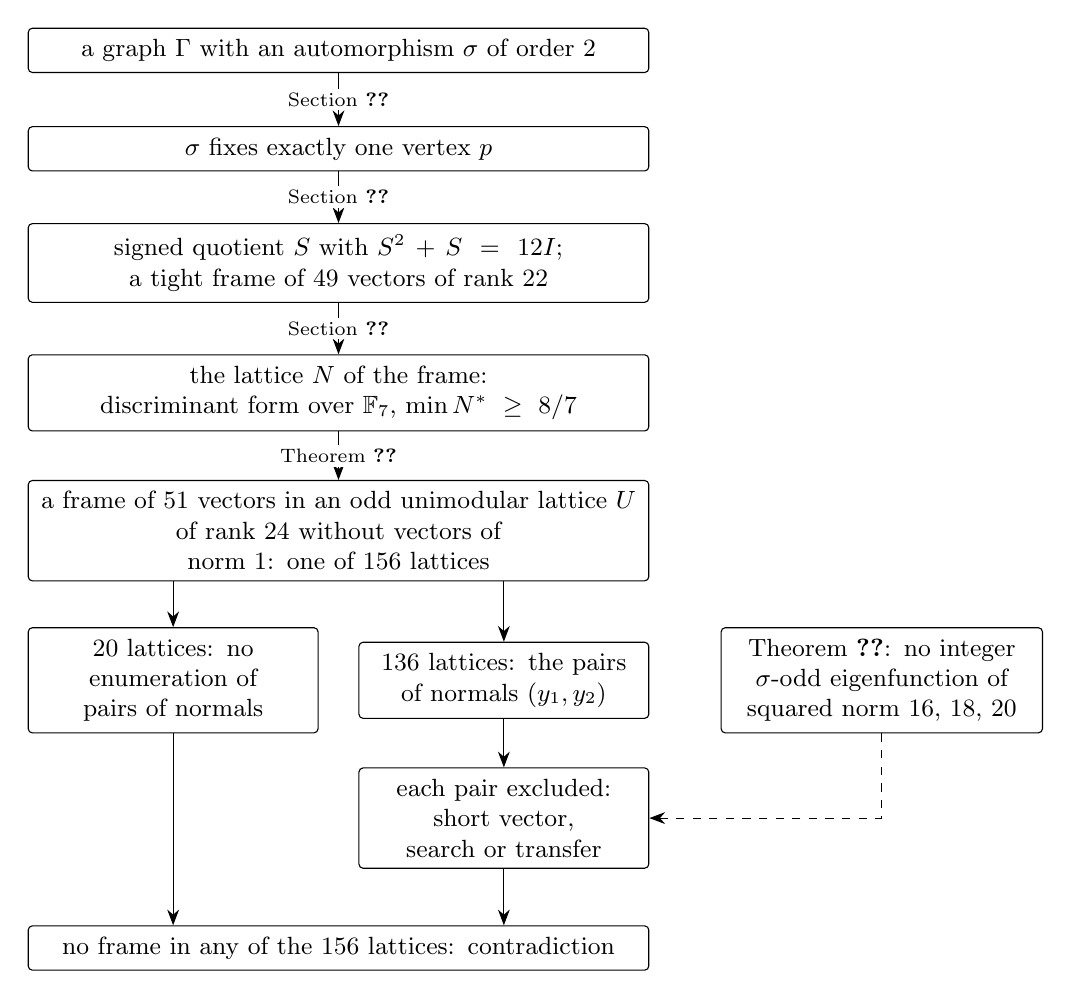
\begin{tikzpicture}[>={Stealth[length=2mm]},
  box/.style={draw, rounded corners=1.5pt, align=center, inner sep=4pt, font=\small, text width=76mm},
  half/.style={draw, rounded corners=1.5pt, align=center, inner sep=4pt, font=\small, text width=34mm},
  side/.style={draw, rounded corners=1.5pt, align=center, inner sep=4pt, font=\small, text width=38mm},
  lab/.style={font=\scriptsize, fill=white, inner sep=1.5pt}]
\node[box] (a) at (0,0) {a graph $\G$ with an automorphism $\s$ of order $2$};
\node[box] (b) at (0,-1.25) {$\s$ fixes exactly one vertex $p$};
\node[box] (c) at (0,-2.7) {signed quotient $S$ with $S^2+S=12I$;\\ a tight frame of $49$ vectors of rank $22$};
\node[box] (d) at (0,-4.35) {the lattice $N$ of the frame:\\ discriminant form over $\F_7$, $\min N^*\ge 8/7$};
\node[box] (e) at (0,-6.1) {a frame of $51$ vectors in an odd unimodular lattice $U$\\ of rank $24$ without vectors of norm
$1$: one of $156$ lattices};
\node[half] (f) at (-2.1,-8.0) {$20$ lattices: no enumeration of pairs of normals};
\node[half] (g) at (2.1,-8.0) {$136$ lattices: the pairs of normals $(y_1,y_2)$};
\node[half] (h) at (2.1,-9.75) {each pair excluded: short vector, search or transfer};
\node[box] (z) at (0,-11.4) {no frame in any of the $156$ lattices: contradiction};
\node[side] (t) at (6.9,-8.0) {Theorem~\ref{thm:T}: no integer $\s$-odd eigenfunction of squared norm $16$, $18$, $20$};
\draw[->] (a) -- node[lab]{Section~\ref{sec:fix}} (b);
\draw[->] (b) -- node[lab]{Section~\ref{sec:frame}} (c);
\draw[->] (c) -- node[lab]{Section~\ref{sec:lattice}} (d);
\draw[->] (d) -- node[lab]{Theorem~\ref{thm:R}} (e);
\draw[->] (e.south -| f.north) -- (f.north);
\draw[->] (e.south -| g.north) -- (g.north);
\draw[->] (g) -- (h);
\draw[->] (f.south) -- (f.south |- z.north);
\draw[->] (h.south) -- (h.south |- z.north);
\draw[->, dashed] (t.south) |- (h.east);
\end{tikzpicture}
\caption{The chain of the proof. The upper chain, through Theorem~\ref{thm:R}, is proved by hand in Sections~\ref{sec:fix}--\ref{sec:env}; the exclusion
of the $156$ lattices (Section~\ref{sec:lattices}) and the lemmas of Theorem~\ref{thm:T} are computer-assisted.}\label{fig:chain}
\end{figure}

\section{Notation}\label{sec:not}

Throughout, $\G$ is a strongly regular graph with parameters $(99,14,1,2)$, $A$ its adjacency matrix, $J$ the all-ones matrix
and $N(x)$ the set of neighbours of a vertex $x$. Thus
\begin{equation}\label{eq:srg}
A^2+A-12I=2J .
\end{equation}
Since $\lambda=1$, the neighbourhood $N(x)$ induces seven disjoint edges, which we call the \emph{blocks} at $x$; every edge
lies in exactly one triangle. A \emph{lattice} is a free $\Z$-module of finite rank with a positive definite rational
symmetric bilinear form $(\ ,\ )$; the \emph{norm} of $v$ is $(v,v)$; $L^*$ denotes the dual lattice. A \emph{root} is a vector of norm $2$; thus ``norm'' always means squared length. A lattice $L$ is \emph{integral} if
$(x,y)\in\Z$ for all $x,y\in L$, that is $L\subseteq L^*$; it is \emph{unimodular} if $L=L^*$, \emph{even} if it is integral
with all norms even, and \emph{odd} if it is integral and not even. A sublattice $M$ of $L$ is \emph{primitive} if $L/M$ has
no torsion. For an integral lattice $L$ the finite group $L^*/L$ is its \emph{discriminant group}; it carries the
\emph{discriminant bilinear form} $(x+L,y+L)\mapsto(x,y)\bmod\Z$. All discriminant forms in this paper are bilinear forms
modulo $\Z$ on vector spaces over $\F_7$, which we identify with $\F_7$-valued forms after multiplication by $7$.

\section{An involution fixes exactly one vertex}\label{sec:fix}

The following proposition is due to Makhnev and Minakova \cite[Theorem~1]{MM}, who obtain it from their classification of
the subgraphs of fixed points. The proof given here counts blocks instead. It has one device in common with theirs, the
integrality of a character of $\s$: they use the eigenspace of dimension $54$ (p.~100 of the Russian original), we use the
complementary one, of dimension $44$.

\begin{proposition}\label{prop:fix}
Let $\s$ be an automorphism of order $2$ of $\G$. Then $\s$ fixes exactly one vertex $p$, it exchanges the two ends of each of
the seven blocks at $p$, and no vertex outside $N(p)$ is adjacent to its image.
\end{proposition}

\begin{proof}
Let $F$ be the set of fixed vertices and $f=|F|$; $f\ge 1$ because $99$ is odd. Let $p\in F$. Then $\s$ permutes the seven
blocks at $p$. A block with a fixed end is fixed pointwise, the other end being the unique common neighbour of $p$ and the
first. Let $s_p$ be the number of blocks fixed pointwise, $t_p$ the number of blocks whose ends are exchanged, and $2r_p$ the
number of blocks sent to another block, so that
\begin{equation}\label{eq:str}
s_p+t_p+2r_p=7 .
\end{equation}
A vertex $z$ at distance $2$ from $p$ is determined by its two neighbours $a,b$ in $N(p)$, which lie in different blocks, and
all $84$ such pairs occur. The vertex $z$ is fixed if and only if $\{a,b\}$ is $\s$-invariant: either $a,b$ are both fixed
($2s_p(s_p-1)$ pairs) or $b=\s a$ lies in another block ($2r_p$ pairs). Counting $p$ and its $2s_p$ fixed neighbours,
\begin{equation}\label{eq:f}
f=1+2s_p^2+2r_p\qquad\text{for every } p\in F .
\end{equation}
Let $a_1$ be the number of vertices $v$ with $v\sim\s v$. For such $v$ the unique common neighbour of $v$ and $\s v$ is a fixed
vertex $p$, and $\{v,\s v\}$ is an exchanged block at $p$; hence $a_1=2\sum_{p\in F}t_p$. A vertex $v$ in a moved block at $p$
is not adjacent to $\s v$; the common neighbours of $v$ and $\s v$ are $p$ and one further vertex, which is fixed; and every
fixed neighbour of $v$ is a common neighbour of $v$ and $\s v$. So $v$ has exactly two fixed neighbours, and the number of
such vertices is $n_2=2\sum_{p\in F}r_p$. These vertices are not fixed and are distinct from those counted by $a_1$:
\begin{equation}\label{eq:a1n2}
a_1+n_2\le 99-f .
\end{equation}
Each triangle fixed pointwise contributes to $s_p$ for its three vertices:
\begin{equation}\label{eq:mod3}
\textstyle\sum_{p\in F}s_p\equiv 0 \pmod 3 .
\end{equation}
Finally, the idempotent of the eigenvalue $-4$ is $\frac17(3I-A)+\frac1{63}J$, and the trace of $\s$ on that eigenspace is an integer (the device of \cite{MM} recalled above):
\begin{equation}\label{eq:trace}
\tfrac17\,(3f-a_1+11)\in\Z .
\end{equation}
By \eqref{eq:str} and \eqref{eq:f} the triple $(s_p,r_p,t_p)$ of a fixed vertex is one of the following. For $f=1$: $(0,0,7)$;
$f=3$: $(0,1,5)$, $(1,0,6)$; $f=5$: $(0,2,3)$, $(1,1,4)$; $f=7$: $(0,3,1)$, $(1,2,2)$; $f=9$: $(1,3,0)$, $(2,0,5)$; $f=11$:
$(2,1,3)$; $f=13$: $(2,2,1)$; $f=19,21,23$: $(3,0,4)$, $(3,1,2)$, $(3,2,0)$; $f=33,35$: $(4,0,3)$, $(4,1,1)$; $f=51,53$:
$(5,0,2)$, $(5,1,0)$; $f=73$: $(6,0,1)$; and $f=99$ for the identity.

For $19\le f\le 73$ the triple is the same at every fixed vertex and $a_1+n_2=2f(t+r)$ equals
$152$, $126$, $92$, $198$, $140$, $204$, $106$, $146$ for $f=19$, $21$, $23$, $33$, $35$, $51$, $53$, $73$, contradicting
\eqref{eq:a1n2}. For $f=11,13$ we get $\sum s_p=22,26$, contradicting \eqref{eq:mod3}. For $f=3,5,7$ let $k$ be the number of
fixed vertices with $s=1$; by \eqref{eq:mod3} $3\mid k$, and $a_1=30+2k$ for $f=3,5$ and $14+2k$ for $f=7$, so that
$3f-a_1+11$ is one of $-10,-16$ $(f=3)$; $-4,-10$ $(f=5)$; $18,12,6$ $(f=7)$, never a multiple of $7$. For $f=9$ let $k$ be the
number of fixed vertices with $s=2$; then $\sum s_p=9+k$, so $k\in\{0,3,6,9\}$, $a_1=10k$ and
$3f-a_1+11\in\{38,8,-22,-52\}$, never a multiple of $7$. All these cases contradict \eqref{eq:trace}. Hence $f=1$ and
$(s_p,r_p,t_p)=(0,0,7)$. Finally, if $u\sim\s u$, the common neighbour of $u$ and $\s u$ is fixed, so it is $p$.
\end{proof}

From now on $\s$ is an involution with fixed vertex $p$. The $14$ vertices of $N(p)$ are called \emph{inner} and the $84$
others \emph{outer}. An outer vertex has exactly two inner neighbours, in two different blocks, and for two blocks $i<j$ the
four non-adjacent pairs of inner vertices have one outer common neighbour each; so the $84$ outer vertices form $42$ orbits,
indexed by the pairs of blocks with a sign (Figure~\ref{fig:local}). This description of the neighbourhood of a vertex,
by seven disjoint edges and the vertices attached to pairs of them, is classical: it is in \cite{W84}, and
\cite[Section~2]{CW} uses it with a labelling of the same kind. For an outer vertex $u$, the set $N(u)\cap N(\s u)$ has two elements, is
$\s$-invariant and does not contain $p$: it is a single orbit $\{v,\s v\}$ of outer vertices.

\begin{figure}[ht]
\centering
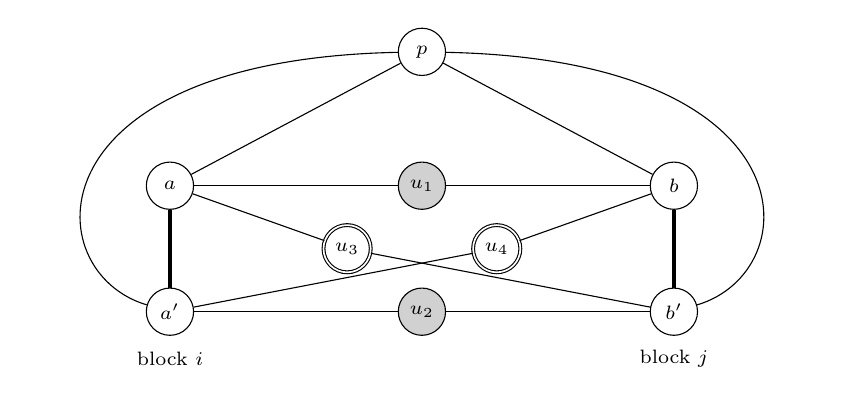
\begin{tikzpicture}[v/.style={circle, draw, inner sep=1.2pt, minimum size=6mm, font=\scriptsize},
  g/.style={v, fill=black!18}, w/.style={v, fill=white}]
\node[w] (p) at (0,3.3) {$p$};
\node[w] (a) at (-3.2,1.6) {$a$};
\node[w] (a2) at (-3.2,0) {$a'$};
\node[w] (b) at (3.2,1.6) {$b$};
\node[w] (b2) at (3.2,0) {$b'$};
\node[g] (u1) at (0,1.6) {$u_1$};
\node[g] (u2) at (0,0) {$u_2$};
\node[w, double] (u3) at (-0.95,0.8) {$u_3$};
\node[w, double] (u4) at (0.95,0.8) {$u_4$};
\draw (p) -- (a);
\draw (p) -- (b);
\draw (p) .. controls (-5.0,3.2) and (-4.9,0.5) .. (a2);
\draw (p) .. controls (5.0,3.2) and (4.9,0.5) .. (b2);
\draw[line width=1.6pt] (a) -- (a2);
\draw[line width=1.6pt] (b) -- (b2);
\draw (a) -- (u1) -- (b);
\draw (a2) -- (u2) -- (b2);
\draw (a) -- (u3) -- (b2);
\draw (a2) -- (u4) -- (b);
\node[font=\scriptsize] at (-3.2,-0.6) {block $i$};
\node[font=\scriptsize] at (3.2,-0.6) {block $j$};
\end{tikzpicture}
\caption{Two of the seven blocks at the fixed vertex $p$ (thick edges) and the four outer vertices attached to them: one
common neighbour for each non-adjacent pair of their ends. The involution $\s$ exchanges $a$ with $a'$ and $b$ with $b'$,
hence $u_1$ with $u_2$ (grey) and $u_3$ with $u_4$ (double circles). With the representatives $a$, $b$, $u_1$, $u_3$ these two
orbits give the columns $e_i+e_j$ and $e_i-e_j$ of the matrix $C$ of Section~\ref{sec:frame}. The other adjacencies of the
outer vertices are not drawn.}\label{fig:local}
\end{figure}

\section{The signed quotient and the frame}\label{sec:frame}

Choose a representative in each of the $49$ orbits of size two. On the space of $\s$-odd functions, with basis the functions
$e_o-e_{\s o}$, the matrix $A$ acts by the symmetric integer matrix
\[
S_{UV}=A[u,v]-A[u,\s v] .
\]
Since $J$ annihilates odd functions, \eqref{eq:srg} gives
\begin{equation}\label{eq:S}
S^2+S=12I .
\end{equation}
The diagonal of $S$ is $-1$ on the $7$ inner orbits and $0$ on the $42$ outer ones, so the trace is $-7$ and the eigenvalues
are $3$ and $-4$ with multiplicities $27$ and $22$. With inner representatives the first ends of the blocks and suitable outer
representatives,
\[
S=\begin{pmatrix}-I_7 & C\\ C^{t} & T\end{pmatrix},
\]
where the $42$ columns of $C$ are the vectors $e_i+e_j$ and $e_i-e_j$ $(i<j)$ of $\Z^7$, and $T$ has zero diagonal and
entries in $\{0,\pm1\}$ with exactly ten nonzero entries in each row (an outer vertex $u$ has $12$ outer neighbours, and
exactly one orbit lies in $N(u)$ entirely). Reading \eqref{eq:S} blockwise,
\begin{equation}\label{eq:blocks}
CC^{t}=12I_7,\qquad CT=0,\qquad T^2+T=12I-C^{t}C .
\end{equation}

Put $H=3I-S$. Then $H^2=7H$ and $\rk H=22$. Let $V$ be the image of $H$, that is the $(-4)$-eigenspace of $S$, and
$u_i=He_i/\sqrt7\in V$. Then $(u_i,u_j)=H_{ij}$: the seven inner vectors $h_c$ have norm $4$ and are pairwise orthogonal, the
$42$ outer vectors $u_o$ have norm $3$, $(h_c,u_o)=-C_{co}$, and the Gram matrix of the $u_o$ is $3I-T$. For $v\in V$,
\begin{equation}\label{eq:tight}
\textstyle\sum_{i=1}^{49}(v,u_i)^2=\tfrac17|Hv|^2=7\,(v,v) ,
\end{equation}
and since $(3e_c;\,C_c^{t})$ is an eigenvector of $S$ for the eigenvalue $3$ by \eqref{eq:blocks},
\begin{equation}\label{eq:rel}
3h_c+\textstyle\sum_{o}C_{co}\,u_o=0\qquad(c=1,\dots,7) .
\end{equation}

\section{The lattice of the frame}\label{sec:lattice}

Let $N$ be the lattice generated by the $49$ vectors $u_i$, let $K=\Z^{49}\cap V$ be the lattice of integer
$(-4)$-eigenvectors of $S$, and $K'$ the lattice of integer $3$-eigenvectors. As $K$ is primitive in $\Z^{49}$, its dual is the projection of $\Z^{49}$ on $V$, that is $K^*=H\Z^{49}/7$: an
integer-valued linear form on $K$ extends to $\Z^{49}$ because $\Z^{49}/K$ is free, it is the product with an integer
vector because $\Z^{49}$ is unimodular, and its restriction to $K$ is the product with the projection of that vector. Hence
\begin{equation}\label{eq:NK}
N=\sqrt7\,K^*,\qquad N^*=K/\sqrt7 ,
\end{equation}
and for $v\in N^*$ the integers $a_i=(v,u_i)$ are the coordinates of the vector $\sqrt7\,v$ of $K$, with $\sum a_i^2=7(v,v)$.

\subsection{The discriminant form}
For $x\in\Z^{49}$ we have $7x=Hx+(S+4I)x\in K\oplus K'$, so $\Z^{49}/(K\oplus K')\cong\F_7^{\,g}$, where $g$ is the rank of
$S-3I$ over $\F_7$. Thus $\det K=7^g$, and the discriminant group of $N$ is $K/7K^*\cong\F_7^{\,22-g}$.

\begin{proposition}\label{prop:witt}
The integer $g$ is even, $g\le 20$, and the discriminant bilinear form of $N$ on $\F_7^{\,22-g}$ is not split: its anisotropic
kernel is a plane. Consequently $N$ has an integral overlattice $N_{\max}\subseteq N^*$ of determinant $49$ whose discriminant
form is the anisotropic plane over $\F_7$.
\end{proposition}

\begin{proof}
The index of $K\oplus K'$ in $\Z^{49}$ is odd, so over $\Z_2$ the lattice $\Z^{49}$ is the orthogonal sum of $K$ and $K'$, both
unimodular, and the projection $c=H\mathbf 1/7$ of the characteristic vector $\mathbf 1$ is a characteristic vector of
$K\otimes\Z_2$. Its norm is $(147-s)/7$ with $s=\mathbf 1^{t}S\mathbf 1$. From \eqref{eq:S},
$588=\mathbf 1^{t}(S^2+S)\mathbf 1=\sum_i r_i^2+s$, where the $r_i$ are the row sums of $S$. The seven inner row sums are odd.
An outer row sum is $r_o=c_o+10-2m_o$, where $c_o\in\{0,2\}$ is the column sum of $C$ and $m_o$ the number of entries $-1$ in
the row of $T$; since $\sum_o c_o/2=21$ and $\sum_o m_o$ is even, the number of outer rows with $r_o\equiv 2\pmod 4$ is odd.
Hence $588\equiv 7+4+s\pmod 8$, so $s\equiv 1$ and $(c,c)\equiv 6\pmod 8$ in $\Z_2$.

Write the $7$-adic Jordan decomposition of $K$ as $1^{\varepsilon_0(22-g)}\,7^{\varepsilon g}$, where the signs
$\varepsilon_0,\varepsilon\in\{\pm1\}$ are the Legendre symbols modulo $7$ of the determinants of the two constituents. The oddity formula
\cite[Ch.~15]{SPLAG} (the signature plus the sum of the $p$-excesses is congruent to the oddity modulo $8$) reads
$22+6g+4[\varepsilon=-1]\equiv 6\pmod 8$. Hence $g$ is even and $\varepsilon=(-1)^{g/2}$; as $\det K=7^g$ exactly,
$\varepsilon_0=\varepsilon$. By \eqref{eq:NK} the discriminant form of $N$ is the form of the unimodular constituent of $K$:
it has dimension $2m=22-g$ and determinant character $\varepsilon_0=(-1)^{g/2}=-(-1)^m$, whereas a hyperbolic form of
dimension $2m$ over $\F_7$ has character $\left(\frac{-1}{7}\right)^m=(-1)^m$. So the form is not split; in particular
$m\ge1$, its Witt index is $m-1$ and its anisotropic kernel is a plane. The preimage in $N^*$ of a totally isotropic subspace
of dimension $m-1$ is the required $N_{\max}$.
\end{proof}

In particular the construction of Section~\ref{sec:env} does not require the value of $g$.

\subsection{The dual minimum}

\begin{proposition}\label{prop:87}
There is no nonzero $a\in\Z^{49}$ with $Sa=-4a$ and $\sum a_i^2\le 7$. Equivalently, the minimum of $N^*$ is at least $8/7$;
equivalently, there is no nonzero integer-valued $\s$-odd function $\varphi$ on the vertices of $\G$ with
$A\varphi=-4\varphi$ and $\sum_x\varphi(x)^2\le 14$.
\end{proposition}

\begin{proof}
If some $|a_i|\ge2$ then $|a_i|=2$ and the other entries have absolute sum at most $3$, whereas row $i$ of $Sa=-4a$ requires
an off-diagonal sum of absolute value $8$ (outer) or $6$ (inner). So $a$ has entries in $\{0,\pm1\}$ and support of size
$m\le 7$. Lift $a$ to an odd function $\varphi$ and put $P=\{\varphi=1\}$, $Q=\s P=\{\varphi=-1\}$, so $|P|=m$. Let $e$ be the
number of edges inside $P$ and $d_i$ the degree of $i\in P$ inside $P$; the equation gives that $i$ has $d_i+4$ neighbours in
$Q$. Count the common neighbours of the pairs of vertices of $P$: the total is $m(m-1)-e$, and the vertices of $P\cup Q$
contribute $\sum_i\bigl[\binom{d_i}{2}+\binom{d_i+4}{2}\bigr]=\sum d_i^2+6e+6m$. So the other vertices contribute
\[
D=m(m-7)-7e-\textstyle\sum d_i^2\ \ge 0 ,
\]
which forces $m=7$, $e=0$ and $D=0$. Then $B_{ij}=[\,i\sim\s j\,]$ is a symmetric $0/1$ matrix on $P$ with row sums $4$, and
$B^2=2I+2J$ because every pair of $P$ has its two common neighbours in $Q$. Its eigenvalues are $4$ and $\pm\sqrt2$, the
latter with equal multiplicities since the characteristic polynomial is rational; so the trace of $B$ is $4$, that is, four
vertices of $P$ are adjacent to their images. By Proposition~\ref{prop:fix} they lie in $N(p)$, and $p\notin P\cup Q$
contributes $\binom42=6$ to $D=0$, a contradiction.
\end{proof}

\section{The envelope}\label{sec:env}

\begin{theorem}\label{thm:R}
Let $\s$ be an automorphism of order $2$ of $\G$. Then there are an odd unimodular lattice $U$ of rank $24$ without vectors of
norm $1$ and vectors $y_1,y_2,h_1,\dots,h_7,u_1,\dots,u_{42}$ of $U$ such that:
\begin{enumerate}[label=\textup{(R\arabic*)},leftmargin=3.2em]
\item $(y_a,y_b)=7\delta_{ab}$, and $y_1,y_2$ are orthogonal to all $h_c$ and $u_o$;
\item $(h_c,h_d)=4\delta_{cd}$, $(u_o,u_o)=3$, and $(u_o,u_{o'})\in\{0,\pm1\}$ for $o\ne o'$, nonzero for exactly ten $o'$;
\item $(h_c,u_o)=-C_{co}$, where the columns of $C$ are the vectors $e_i\pm e_j$ $(i<j)$ of $\Z^7$;
\item $3h_c+\sum_oC_{co}u_o=0$ for every $c$;
\item for every real vector $v$: $\ \sum_c(v,h_c)^2+\sum_o(v,u_o)^2+(v,y_1)^2+(v,y_2)^2=7\,(v,v)$;
\item $\Z y_1+\Z y_2$ is primitive in $U$, and every $v\in U$ outside it satisfies
$E(v):=7(v,v)-(v,y_1)^2-(v,y_2)^2\ge 8$;
\item for every $v\in U$, the $49$ integers $(v,h_c)$, $(v,u_o)$ are the values on orbit representatives of an
integer-valued $\s$-odd function $\varphi_v$ with $A\varphi_v=-4\varphi_v$ and $\sum_x\varphi_v(x)^2=2E(v)$;
\item every nonzero vector $w$ of the real span of the $h_c$, $u_o$ whose inner products with all $h_c$, $u_o$ are integers
has $(w,w)\ge 8/7$.
\end{enumerate}
\end{theorem}

\begin{proof}
Let $N_{\max}$ be as in Proposition~\ref{prop:witt} and $\Pl=\Z r_1+\Z r_2$ with $(r_a,r_b)=7\delta_{ab}$. The discriminant
form of $\Pl$ is the anisotropic plane over $\F_7$, because $-1$ is not a square modulo $7$. Nondegenerate forms over $\F_7$
are classified by dimension and determinant ($7$ being odd; \cite[Ch.~IV, \S1.7]{Serre}), and an anisotropic plane and its negative both have square determinant; so the
discriminant forms of $N_{\max}$ and $\Pl$ are anti-isometric. Gluing along the graph of an anti-isometry \cite[\S1]{Nik}, \cite[Ch.~4, \S3]{SPLAG} (for the discriminant bilinear forms modulo $\Z$; the lattices here are odd, and no quadratic form modulo $2\Z$ is
involved) gives an integral lattice $U$ containing $N_{\max}\oplus\Pl$ with index $49$, of rank $24$ and determinant $49\cdot49/49^2=1$, in which
$N_{\max}$ and $\Pl$ are primitive; $U$ is odd since it contains vectors of norm $3$. Put $y_a=r_a$. Properties (R1)--(R4)
are those of Section~\ref{sec:frame}, (R5) is \eqref{eq:tight} together with the orthogonal basis $y_1,y_2$ of $V^\perp$, and
(R8) is Proposition~\ref{prop:87}.

For $v\in U$ the projection of $v$ on $V$ lies in $N_{\max}^*\subseteq N^*$; by \eqref{eq:NK} its $49$ inner products with the
frame form a vector $a\in K$ with $\sum a_i^2=E(v)$, and the lift of $a$ to the vertices is the function $\varphi_v$ of (R7).
If $a=0$ then $v\in U\cap V^\perp=\Pl$. Otherwise $E(v)\ge8$ by (R8); this is (R6). In particular a vector of norm $1$ would
have $E\le7$, hence lie in $\Pl$, whose minimum is $7$.
\end{proof}

There are exactly $156$ odd unimodular lattices of rank $24$ without vectors of norm $1$, up to isometry
\cite{Bor}. We call a system of $51$ vectors with the properties (R1)--(R8), for some pair $(\G,\s)$, a \emph{frame} in $U$,
and $y_1,y_2$ its \emph{normals}. The pair $(\G,\s)$ enters only through (R7), and (R7) is used below only through
Theorem~\ref{thm:T}. Theorem~\ref{thm:main} follows from Theorem~\ref{thm:R} and:

\begin{theorem}\label{thm:B}
None of the $156$ odd unimodular lattices of rank $24$ without vectors of norm $1$ contains a frame.
\end{theorem}

The rest of this section records consequences of (R1)--(R8) that are used repeatedly.

\begin{lemma}\label{lem:gen}
In a frame, the $42$ vectors $u_o$ generate the lattice $N$ generated by all $49$ vectors $h_c$, $u_o$. The graph on the $u_o$
in which $u_o$, $u_{o'}$ are joined when $(u_o,u_{o'})=\pm1$ is connected.
\end{lemma}

\begin{proof}
Let $M$ be the lattice generated by the $u_o$. By (R4), $3h_c\in M$. Polarising (R5) and applying it to $u_o$ gives
\begin{equation}\label{eq:pol}
\textstyle\sum_cC_{co}h_c=-4u_o+\sum_{p\ne o}(u_o,u_p)\,u_p\in M ;
\end{equation}
the two columns of $C$ for the pair $\{i,j\}$ give $h_i+h_j$ and $h_i-h_j$, hence $2h_i\in M$ and $h_i\in M$. Now define
$T_{oo'}=-(u_o,u_{o'})$ for $o\ne o'$ and $T_{oo}=0$. Pairing \eqref{eq:pol} with $u_{o'}$, $o'\ne o$, gives
$\sum_{o''}T_{oo''}T_{o''o'}+T_{oo'}=-(C^tC)_{oo'}$. If the graph were the disjoint union of two nonempty parts, the left side
would vanish for $o$, $o'$ in different parts, whereas $(C^tC)_{oo'}=\pm1$ when $o$ and $o'$ share exactly one block. So two
orbits sharing exactly one block lie in the same part; but the graph ``sharing exactly one block'' on the $42$ orbits is
connected.
\end{proof}

\begin{lemma}\label{lem:indec}
A lattice containing a frame is indecomposable.
\end{lemma}

\begin{proof}
Let $U=L_1\oplus L_2$ with $L_1,L_2\ne0$. The summands are unimodular without vectors of norm $1$, so a vector of norm $3$
lies in one of them, and vectors of different summands are orthogonal. By Lemma~\ref{lem:gen} all the $u_o$ lie in one
summand, say $L_1$, and so do the $h_c$. Then $L_2$ is orthogonal to the $49$ vectors, hence contained in the plane of
$y_1,y_2$; but a unimodular lattice of rank $1$ or $2$ contains a vector of norm $1$.
\end{proof}

\begin{definition}\label{def:shadow}
Let $U$ be an odd unimodular lattice of rank $24$ and $U_0$ its sublattice of vectors of even norm. The quotient
$U_0^*/U_0$ has four classes: $U_0$, $U\setminus U_0$ and two classes $S_1$, $S_2$, whose union is the \emph{shadow}
$\{z/2: z \text{ characteristic}\}$ of $U$. The vectors of norm $2$ of the shadow are the \emph{new roots} of $U$: they are the
roots of the even unimodular lattices $U_0\cup S_j$ that are not in $U$. (The shadow and these four classes are described in \cite[\S2, p.~386]{CS90}; in rank $24$ both $U_0\cup S_1$ and
$U_0\cup S_2$ are even unimodular lattices, the two \emph{even neighbours} of $U$ \cite{Bor}.)
\end{definition}

\begin{lemma}\label{lem:newroots}
Let $\beta$ be a new root of a lattice containing a frame. Then $w(\beta):=\sum_c(\beta,h_c)^2\in\{1,3\}$, the integers
$(\beta,h_c)$ have absolute value at most $1$, and at most one of the $44$ vectors $u_o$, $y_a$ has
$|(\beta,\cdot)|=3/2$; if there is one then $w(\beta)=1$, otherwise $w(\beta)=3$.
\end{lemma}

\begin{proof}
With $z=2\beta$ characteristic, the products $(z,u_o)$ and $(z,y_a)$ are odd and $(z,h_c)$ is even. In (R5) for $v=\beta$
the right side is $14$; the $44$ terms from $u_o,y_a$ are at least $1/4$ each, a product of absolute value $3/2$ adds $2$ and
a larger one at least $6$. Hence $w(\beta)=3-2\cdot\#\{\text{products equal to }\pm 3/2\}\ge0$.
\end{proof}

\begin{lemma}\label{lem:char}
For a characteristic vector $z$ of norm $16$ of a lattice containing a frame, $(z,y_1)^2+(z,y_2)^2\le66$.
\end{lemma}

\begin{proof}
$E(z)=112-Y$ with $Y=(z,y_1)^2+(z,y_2)^2\equiv2\pmod8$, and $E(z)=\sum_o(z,u_o)^2+4\sum_cb_c^2$ with $(z,h_c)=2b_c$ and
the $(z,u_o)$ odd. Modulo $8$ this gives $6\equiv42+4\sum b_c^2$, so $\sum b_c^2$ is odd, $E(z)\ge46$ and $Y\le66$.
\end{proof}

\begin{lemma}[Twins]\label{lem:twin}
Let $y_1,y_2$ be the normals of a frame in $U$, $M=U\cap\{y_1,y_2\}^\perp$ and $\Pl=\Z y_1+\Z y_2$. Let $U'$ be any
unimodular lattice containing $M\oplus\Pl$ in which $M$ and $\Pl$ are primitive. Then $U'$ is odd, has no vector of norm $1$,
and the same $51$ vectors form a frame in $U'$.
\end{lemma}

\begin{proof}
The frame vectors lie in $M\oplus\Pl$, so (R1)--(R5) and (R8) hold in $U'$. As $M$ is primitive in the unimodular lattices
$U$ and $U'$, both project onto $M^*$ in the space $V$ spanned by $M$. Since $E(v)$ is $7$ times the norm of the projection
of $v$ on $V$, and the function $\varphi_v$ depends only on that projection, (R6) and (R7) pass from $U$ to $U'$. A vector of
norm $1$ of $U'$ would have $E\le7$ and lie in $\Pl$.
\end{proof}

\section{Energy and eigenfunctions of small norm}\label{sec:energy}

By (R5) the energy $E(v)$ of $v\in U$ is $7$ times the squared norm of the projection of $v$ on the space of the frame. It is
a non-negative integer, it is unchanged when a multiple of $y_1$ or $y_2$ is added to $v$, and it vanishes exactly on
$\Z y_1+\Z y_2$. By (R7), for $E\ge1$ a statement ``there is no integer $\s$-odd eigenfunction of squared norm $2E$''
forbids every vector of energy $E$ in every lattice containing a frame.

\begin{theorem}[Lemmas $T_{16}$, $T_{18}$, $T_{20}$]\label{thm:T}
Let $\s$ be an automorphism of order $2$ of $\G$. There is no integer-valued function $\varphi$ on the vertices of $\G$ with
$\varphi\circ\s=-\varphi$, $A\varphi=-4\varphi$ and $\sum_x\varphi(x)^2\in\{16,18,20\}$.
\end{theorem}

The three proofs are long and computer-assisted; they are given in full in the supplement \cite{repo}
(\texttt{lemma/T16\_PROOF.md}, \texttt{T18\_PROOF.md}, \texttt{T20\_PROOF.md}). They follow the scheme of
Proposition~\ref{prop:87}. First, $\varphi$ takes the values $0,\pm1$. With $S^+=\{\varphi=1\}$ and $S^-=\s S^+$, each vertex
of $S^+$ has four more neighbours in $S^-$ than in $S^+$, and the count of common neighbours bounds the number of edges
inside $S^+$. The bipartite graph between $S^+$ and $S^-$ is then one of finitely many \emph{support structures}: for the
squared norm $16$, the complements of the cube and of the Wagner graph; for $20$, nine configurations, sorted by the number
of support vertices adjacent to $p$. Each structure is excluded, by hand where possible, and otherwise by an exhaustive
search over the vertices outside the support in which every rejection is exact: a count of common neighbours; an integer
vector on which one of the positive semidefinite matrices $9(3I-A)+J$ and $11(4I+A)-2J$ would take a negative value; or, for
one family of $T_{18}$ and at sixteen nodes of the first program of $T_{20}$, an exact computation of a rank that would
exceed $22$ (the $\s$-odd part of $9(3I-A)+J$ has rank at most $22$). For $T_{20}$ the second program closes these sixteen
nodes by its own search, without the rank bound. The largest group of searches of $T_{20}$ visits $1.58\cdot10^7$ nodes
from $615{,}405$ starting configurations. How these
computations were verified is described in Section~\ref{sec:verif}.

\begin{corollary}\label{cor:E11}
Let $U$ contain a frame. Then $E(v)\ge 11$ for every $v\in U$ outside $\Z y_1+\Z y_2$.
\end{corollary}

Adding multiples of $y_1,y_2$ we may assume $|(v,y_a)|\le3$; then $(v,v)=(E(v)+a^2+b^2)/7$ with $a=(v,y_1)$, $b=(v,y_2)$ and
$a^2+b^2\le18$, so $(v,v)\le4$ when $E(v)\le10$. Going through the norms $2$, $3$, $4$ shows that the vectors of energy $8$,
$9$, $10$ are, up to $\Z y_1+\Z y_2$, exactly the following \emph{witnesses}:
\begin{itemize}[leftmargin=3.5em]
\item[(W8)] a vector of norm $3$ with $\{|a|,|b|\}=\{2,3\}$;
\item[(W9)] a root with $\{|a|,|b|\}=\{1,2\}$;
\item[(W10)] a root with $\{|a|,|b|\}=\{0,2\}$, or a vector of norm $4$ with $|a|=|b|=3$.
\end{itemize}
In the same way a vector of energy at most $7$ outside $\Z y_1+\Z y_2$ has a representative of norm $2$ or $3$. So (R6) and
Corollary~\ref{cor:E11} are finite tests on the vectors of norm $2$, $3$, $4$ of $U$: a pair $(y_1,y_2)$ with a witness is
the pair of normals of no frame, and exhibiting the witness proves it. The numbers of vectors of these norms satisfy $N_4=196560-24N_2-24N_3$, and $N_3=4096$ (the specialisation to rank $24$ of the expansions of the theta series
of a unimodular lattice and of its shadow, \cite[\S2]{CS90}); the first identity is used to certify that the lists are complete.

\begin{corollary}\label{cor:Y1}
Let $U$ contain a frame. Then every root $r$ of $U$ has $|(r,y_1)|\le1$ and $|(r,y_2)|\le1$. In particular, if $U$ has a root
$r$ with $(r,y)=\pm2$ for some vector $y$ of norm $7$, then $y$ is a normal of no frame of $U$, whatever the other normal.
\end{corollary}

\begin{proof}
$E(r)=14-a^2-b^2\ge8$ gives $a^2+b^2\le6$; if $|a|=2$ then $E(r)=10-b^2\in\{9,10\}$, contradicting
Corollary~\ref{cor:E11}.
\end{proof}

\section{The 156 lattices}\label{sec:lattices}

This section describes the proof of Theorem~\ref{thm:B}. Lattices are referred to by their number $000$--$155$ in the table
of Appendix~\ref{app:table}, in which they are ordered by increasing number of roots, and by their root system.

\subsection{The lattices}
The $156$ lattices are given by generators. For each of them the following was computed twice, first by programs with
floating-point steps (in the enumeration of short vectors and in the ranks of the root components), then by an independent
program in exact arithmetic: the determinant is $1$, the lattice is odd, it has no vector of norm $1$, and its root system
is the one of the classification. The root system separates all but seven pairs of lattices, and those are separated by
their two even neighbours (also recomputed exactly). So the data are $156$ pairwise non-isometric lattices of the list,
hence all of them by \cite{Bor}.
% Exact recomputation: Codex, 07/10, q/codex_exact_lattice_identity.py, measures/codex_exact_lattice_identity.json,
% lemma/t20_CODEX/EXACT_LATTICE_IDENTITY.md (on master since bd4e1f021; summary read: all_156_exact_input_checks_passed
% true, pairwise_nonisometric true, 7 pairs with equal root types, 156 records).

\subsection{Twenty lattices excluded without enumerating pairs of normals}

\begin{proposition}[Packing]\label{prop:pack}
Let $U$ contain a frame, let $j\in\{1,2\}$ and let $R_j$ be the set of new roots in the class $S_j$. For a vector $x$ of
norm $3$ let $m_j(x)$ be the number of $\beta\in R_j$ with $|(\beta,x)|=3/2$. Then:
\begin{enumerate}[label=\textup{(\alph*)}]
\item $\sum_{o=1}^{42}m_j(u_o)\le|R_j|$. In particular the sum of the $42$ smallest values of $m_j$ on the vectors of norm
$3$ taken up to sign is at most $|R_j|$, and a vector $x$ of norm $3$ can be one of the $\pm u_o$ only if $m_j(x)$ plus the
sum of the $41$ smallest values of $m_j$ on the other classes is at most $|R_j|$ \textup{(}$x$ is then called
\emph{admissible}\textup{)}.
\item If $\mathcal A$ is a set of vectors of norm $3$ containing all the $u_o$ and $L$ the lattice it generates, then
$\rk L\ge22$, and the vectors $w$ of the real span of $L$ with $(w,L)\subseteq\Z$ and $(w,w)<8/7$ span, together with
$L^\perp$, a space of dimension at most $2$.
\end{enumerate}
\end{proposition}

\begin{proof}
(a) By Lemma~\ref{lem:newroots} a new root is met at $\pm3/2$ by at most one $u_o$, so the $42$ sets counted by the
$m_j(u_o)$ are pairwise disjoint subsets of $R_j$; and the $u_o$ are pairwise distinct up to sign by (R2). (b) By
Lemma~\ref{lem:gen}, $L$ contains $N$, of rank $22$. Let $w$ be such a vector. It has integer products with the $h_c$ and
$u_o$, and so has its projection on the span $V$ of the frame, whose norm is less than $8/7$; by (R8) this projection is
zero, so $w\in V^\perp$. Also $L^\perp\subseteq N^\perp=V^\perp$, which has dimension $2$.
\end{proof}

For every lattice one has $m_1=m_2$ on the vectors of norm $3$ (if $(\beta,x)=3/2$ then $x-\beta$ is a new root of the other
class with the same product). Table~\ref{tab:pack} gives the outcome of the computation for $18$ lattices: for fourteen of
them the first inequality of (a) fails; for the four others the lattice generated by the admissible vectors violates (b).

\begin{table}[ht]
\centering\small
\begin{tabular}{llrr@{\qquad\quad}llrr}
\toprule
lattice & roots & $\Sigma_{42}$ & $\min|R_j|$ & lattice & roots & $\Sigma_{42}$ & $\min|R_j|$\\
\midrule
094 & $d_5^4$ & 84 & 80 & 147 & $a_{15}d_8$ & 84 & 32\\
128 & $a_9e_6d_6a_1$ & 84 & 64 & 148 & $a_{15}e_7a_1$ & 168 & 64\\
129 & $e_6^2d_5^2$ & 84 & 64 & 150 & $d_8e_7^2a_1^2$ & 168 & 64\\
133 & $a_{13}d_6a_3a_1$ & 168 & 128 & 151 & $d_{12}d_8d_4$ & 336 & 128\\
136 & $a_{11}^2$ & 84 & 48 & 152 & $e_8d_8^2$ & 672 & 256\\
142 & $d_{10}d_6^2a_1^2$ & 168 & 128 & 154 & $a_{23}$ & 252 & 48\\
144 & $a_{16}a_7$ & 168 & 104 & 155 & $d_{16}d_8$ & 672 & 128\\
\bottomrule
\end{tabular}

\medskip
\begin{tabular}{llr@{\qquad\quad}llr}
\toprule
lattice & roots & dimension & lattice & roots & dimension\\
\midrule
117 & $d_8d_4^4$ & 8 & 145 & $d_8^3$ & 8\\
134 & $d_9a_7^2$ & 9 & 146 & $d_8^3$ & 24\\
\bottomrule
\end{tabular}
\caption{The packing test. Above: the sum $\Sigma_{42}$ of the $42$ smallest values of $m_j$ exceeds the number of new roots
of a class. Below: the dimension spanned by the short dual vectors of Proposition~\ref{prop:pack}(b), for $\mathcal A$ the
set of admissible vectors, exceeds $2$.}\label{tab:pack}
\end{table}

\begin{proposition}\label{prop:153}
The lattices $153$ $($root system $d_{12}^2)$ and $152$ $($root system $e_8d_8^2)$ contain no frame.
\end{proposition}

\begin{proof}
The lattices $D_{12}^+\oplus D_{12}^+$ and $E_8\oplus O_{16}$, where $D_{12}^+$ and $O_{16}$ are the odd unimodular lattices
of rank $12$ and $16$ with root systems $d_{12}$ and $d_8^2$, are odd unimodular of rank $24$ without vectors of norm $1$,
with root systems $d_{12}^2$ and $e_8d_8^2$. Each of these root systems occurs once in the list, so these are the lattices
$153$ and $152$. They are decomposable; apply Lemma~\ref{lem:indec}.
\end{proof}

\begin{proposition}\label{prop:143}
The lattice $143$ $($root system $a_{15}a_8)$ contains no system of vectors satisfying \textup{(R2)} and \textup{(R5)}.
\end{proposition}

\begin{proof}
Summing (R5) over an orthonormal basis of a subspace $W$ gives $\sum_f|P_Wf|^2=7\dim W$, the sum being over the $51$ frame
vectors and $P_W$ the orthogonal projection. Let $W$ be the span of the component $a_8$ $(\dim W=8)$ and $\ell$ the line
orthogonal to all roots. The vectors of $U$ orthogonal to the roots are the multiples of a primitive vector $z$ with
$(z,z)=144$, and the $4096$ vectors $x$ of norm $3$ are of three kinds:
\begin{center}\small
\begin{tabular}{rrrr}
\toprule
$(x,z)^2$ & $|P_Wx|^2$ & $|P_\ell x|^2$ & number\\
\midrule
$81$ & $0$ & $9/16$ & $1120$\\
$169$ & $8/9$ & $169/144$ & $288$\\
$9$ & $2$ & $1/16$ & $2688$\\
\bottomrule
\end{tabular}
\end{center}
In each case $4|P_Wx|^2+16|P_\ell x|^2\ge9$. Summing over the $42$ vectors $u_o$ gives
$378\le4\cdot56+16\cdot7=336$, a contradiction.

The table follows from the description of $U$ as a gluing of $A_{15}\oplus A_8\oplus\Z z$: writing
$x=x_{15}+x_8+\frac{t}{144}z$ with $t=(x,z)$, the component $x_{15}$ lies in the class $5t$ of $A_{15}^*/A_{15}\cong\Z/16$ and
$x_8$ in the class $7t$ of $A_8^*/A_8\cong\Z/9$ (for suitable generators), the norms in the class $i$ of $A_n^*$ are
$i(n+1-i)/(n+1)+2k$, $k\ge0$, and among the $|t|\le20$ norm $3$ occurs exactly for $t=\pm3$ $(\frac{15}{16}+2+\frac1{16})$,
$t=\pm9$ $(\frac{39}{16}+0+\frac{9}{16})$ and $t=\pm13$ $(\frac{15}{16}+\frac89+\frac{169}{144})$, with
$2\cdot16\cdot84$, $2\cdot560$ and $2\cdot16\cdot9$ vectors. The details, and the exact verification of the gluing on the
data, are in \texttt{lemma/upstream/LATTICE\_143.md} of \cite{repo}.
\end{proof}

Propositions~\ref{prop:pack}, \ref{prop:153} and~\ref{prop:143} exclude the $20$ lattices $094$, $117$, $128$, $129$, $133$,
$134$, $136$, $142$--$148$, $150$--$155$; lattice $152$ is covered twice.

\subsection{Enumeration of the pairs of normals}\label{ssec:enum}
For the other $136$ lattices the pairs $(y_1,y_2)$ of orthogonal vectors of norm $7$ are enumerated up to automorphisms of $U$
and signs. Only pairs satisfying the following necessary conditions are produced; they are instances of (R6) and of
Lemma~\ref{lem:newroots}: for every root $\alpha$, $(\alpha,y_1)^2+(\alpha,y_2)^2\in\{0,1,2,4,5\}$; for every vector $x$ of
norm $3$, $|(x,y_a)|\le3$ and not both equal to $3$; for every new root $\beta$, $|(\beta,y_a)|\le3/2$ and not both equal to
$3/2$; and no nonzero vector of the dual of $U\cap\{y_1,y_2\}^\perp$ has norm less than $8/7$.

Reflections in roots are automorphisms of $U$. So $y_1$ may be taken dominant for the Weyl group $W(R)$ of the root system,
and then $y_2$ dominant for the stabiliser of $y_1$ in $W(R)$, which is generated by the simple reflections fixing $y_1$ \cite[\S1.12]{Hum}. The
dominant vectors are obtained from their projections on the root components (dominant weights with labels at most $2$, by
the condition on roots, combined according to the glue classes) and from their component in the orthogonal complement of the
roots, enumerated by a Fincke--Pohst procedure \cite{FP} with exact final tests. (The final tests certify the vectors that
are kept; that none is missed rests on the correctness of the procedure, except for the vectors of norm $2$, $3$, $4$,
whose lists are certified complete by their counts, Section~\ref{sec:verif}.) The pairs are further reduced by a group of diagram
automorphisms, each verified to preserve $U$; using a subgroup of the automorphism group is always sound. We call this
procedure the \emph{main enumeration}; it is used for $102$ lattices. The conditions
for a frame are symmetric in $y_1,y_2$ and the enumeration contains both orders, so a pair is skipped when $I(y_1)>I(y_2)$,
where $I$ is an invariant of the orbit of a vector (the sum of $(\alpha,y)^2$ over the roots, and the sorted numbers of new
roots of the two classes met at $3/2$). For the odd Leech lattice $(000)$ and the lattices $001$, $002$, $004$, $010$, with
root systems $a_1^8$, $a_1^{12}$, $a_1^{16}$, $a_1^{24}$, the pairs are produced by separate programs: $141$ classes for the
odd Leech lattice, and lists in coordinates of the Niemeier lattice with root system $A_1^{24}$ for the four others.

The completeness of the pair enumeration was compared with an independent enumerator (all vectors of norm $7$ by
Fincke--Pohst, its own Weyl reduction, no diagram automorphisms) on four lattices: $140$, $135$, $141$ and $064$, the last
one with roots that do not span the space. The two sets of pairs coincide in each case ($288$, $464$, $331$ and
$1{,}050{,}528$ pairs). For this comparison the producer was run without diagram automorphisms; the reduction by these
automorphisms, used in the main enumeration, is not covered by it: it rests on the verification of each automorphism (it preserves the
Gram matrix and permutes the simple roots) and on the few lines of the program that select one representative per orbit.
For the other lattices completeness rests on the argument above and on the program that produces the pairs.

\subsection{Exclusion of a pair}\label{ssec:excl}
Each pair is excluded in one of the following ways.

\smallskip\noindent\emph{(i) At once.} A vector of energy at most $7$, contradicting (R6); a witness (W8), contradicting
$T_{16}$; or a characteristic vector of norm $16$ violating Lemma~\ref{lem:char}.

\smallskip\noindent\emph{(ii) By a witness (W9) or (W10)}, contradicting $T_{18}$ or $T_{20}$. Each such pair has a
certificate: the vectors $y_1$, $y_2$ and the witness in coordinates; a separate program checks in exact arithmetic that the
three vectors lie in $U$ and have the required norms and inner products.

\smallskip\noindent\emph{(iii) By search.} The candidates for the $h_c$ are the vectors of norm $4$ orthogonal to
$y_1,y_2$ with $|(\beta,h)|\le1$ for every new root $\beta$. By Lemma~\ref{lem:newroots} every new root $\beta$ must be
\emph{covered}: $w(\beta)=1$ if a normal meets $\beta$ at $3/2$, and $w(\beta)\in\{1,3\}$ otherwise, with $w(\beta)=1$ only
if some $u_o$ meets $\beta$ at $3/2$. The search looks for seven pairwise orthogonal candidates with these coverages,
branching on a new root that still needs covering, and discards a partial choice as soon as a necessary condition fails.
The conditions used are consequences of (R1)--(R5) and of the lemmas of Section~\ref{sec:env}. The main ones are: for every
pair of chosen $h$ there must remain candidates for both vectors $u_o$ of that pair of blocks (vectors of norm $3$,
orthogonal to $y_1,y_2$ and to the other chosen $h$, with the products (R3)); $h_1+\dots+h_7\in2U$ (sum (R4) over $c$: every
column of $C$ has even sum); for each $c$ the twelve vectors $u_o$ with $C_{co}\neq0$, suitably signed, sum to $3h_c$, which
constrains their products with every new root; and finally the $42$ vectors must be distinct, with a Gram matrix $3I-T$
satisfying \eqref{eq:blocks}. Reflections of $U$ fixing the vectors already chosen are used to identify equivalent branches.
A search that exceeds a preset number of nodes is reported as incomplete and is not an exclusion; no pair was left in that
state.

\smallskip\noindent\emph{(iv) By transfer to a twin.} Let $U'$ be the unimodular lattice of Lemma~\ref{lem:twin} obtained by
composing the gluing map of $U$ with the isometry $\left(\begin{smallmatrix}2&2\\-2&2\end{smallmatrix}\right)$ of the
discriminant form of $\Z y_1+\Z y_2$; its roots are obtained from the vectors of norm $2$, $3$, $4$ of $U$. The pair
$(y_1,y_2)$ hosts a frame in $U$ if and only if it does in $U'$, and $U'$ is a lattice of the list. The program uses this in
three forms, tried in this order.
\begin{enumerate}[label=\textup{(\alph*)},leftmargin=2.4em]
\item \emph{Status.} If all the lattices of the list with the root system of $U'$ were already recorded as containing no
frame when the pair was treated, the pair is excluded.
\item \emph{More roots.} Otherwise, if $U'$ has strictly more roots than $U$, the pair is set aside, and it is excluded when
all the lattices with more roots than $U$ are. This is a descending induction on the number of roots; it does not require
$U'$ to be identified, only its number of roots, as computed by the program, to exceed that of $U$. The dependencies it
creates between lattices ($1{,}622$ of them) contain no cycle.
\item \emph{Same lattice.} Otherwise, if $U'$ has the root system of $U$ and this root system occurs once in the list, then
$U'\cong U$, and the pair is replaced by its image in $U$ when an invariant key of the pair decreases strictly.
\end{enumerate}
Forms (a) and (c) need the root system of $U'$; the program reads it from the numbers of roots of the components and from
their ranks, computed in floating point. Form (a) moreover depends on the order in which the lattices were treated. What
this implies for the proof is discussed in Section~\ref{sec:verif}.

\medskip
\smallskip\noindent\emph{The logical procedure.} For a lattice $U$ of the list the certification therefore reads as
follows; this is the logical order, not the order in which the campaign was run. (1) List the pairs of normals
$(y_1,y_2)$ up to the symmetries of Section~\ref{ssec:enum}. (2) For each pair, look for a vector contradicting (R6),
Lemma~\ref{lem:char} or Theorem~\ref{thm:T}; if there is one, the pair is excluded and the vector is its witness. (3)
Otherwise, compute the roots of the twin lattice; if it has more roots than $U$, the pair is excluded by induction, and if
it is $U$ itself with a smaller key, the pair is replaced by its image (the campaign also used the status form (a) above,
which is the part discussed in Section~\ref{sec:verif}). (4) Otherwise search for the seven vectors $h_c$ and
then for the $42$ vectors $u_o$; the pair is excluded if the search ends without a frame. (5) A search stopped by a limit
excludes nothing. The lattice is excluded when all its pairs are.

\medskip
The correspondence between these rules and the program, rule by rule, with the derivation of each rule from the properties
of a frame, is the audit \texttt{lemma/upstream/AUDIT\_ENGINE\_RULES.md} of \cite{repo}.

\subsection{Results}\label{ssec:results}

Table~\ref{tab:methods} summarises how the $156$ lattices are treated; the paragraphs below give the details, and
Appendix~\ref{app:table} the numbers lattice by lattice.

\begin{table}[ht]
\centering\small
\begin{tabular}{p{88mm}rr}
\toprule
treatment & lattices & pairs\\
\midrule
arguments on the lattice (Propositions~\ref{prop:pack}, \ref{prop:153}, \ref{prop:143}) & $20$ & ---\\
main enumeration; exclusion at once, by search or by transfer & $91$ & $220{,}260{,}576$\\
the same with witnesses (W9), (W10) and certificates: $11$ lattices of the main enumeration and the lattices $001$,
$002$, whose pairs are listed by a separate program & $13$ & $373{,}439{,}131$\\
odd Leech lattice: linear certificates and searches & $1$ & $141$ classes\\
lattices $004$, $010$: lists of pairs & $2$ & $420{,}345$\\
lists of pairs (September), then lemmas and a complete second run & $29$ & $6{,}713{,}853$\\
\midrule
 & $156$ & \\
\bottomrule
\end{tabular}
\caption{The treatment of the $156$ lattices. The main enumeration covers $102$ lattices ($91+11$). For the odd Leech
lattice the unit is a class of pairs, not a pair.}\label{tab:methods}
\end{table}

\subsubsection*{$91$ lattices of the main enumeration} For these lattices every pair goes through (i), (iii) or (iv); the
enumeration itself does not use the lemmas $T_{18}$, $T_{20}$. They enter for these lattices in one way only: for the
representatives $y_1$ whose records come from a program version that was not recorded and that were not run again, the
exclusion rests on Corollary~\ref{cor:Y1} (Section~\ref{sec:verif}, item 3 of the paragraph on the search). The records
were recounted: every representative $y_1$ is covered exactly once, and
there are $220{,}260{,}576$ pairs, of which $97{,}628{,}147$ are excluded at once, $22{,}702{,}398$ by search,
$6{,}107{,}330$ by transfer, $93{,}822{,}540$ are skipped by the symmetry in $(y_1,y_2)$, and $161$ were first reported
incomplete and then excluded by a second search with a larger limit.

\subsubsection*{The $13$ lattices with the smallest root systems} $(001$--$003$, $005$--$009$, $011$--$015)$. Here the
searches are long, and a pair with a witness (W9) or (W10) is set aside instead of searched: $5{,}190{,}752$ pairs are
excluded through $T_{18}$ and $2{,}508{,}295$ through $T_{20}$, each with its certificate (ii); the other pairs are excluded
by (i), (iii), (iv). For one representative $y_1$ of lattice $003$ $(a_2^2a_1^{10})$ the enumeration of the $y_2$ did not
terminate; this $y_1$ has a root $r$ with $(r,y_1)=-2$ and is excluded by Corollary~\ref{cor:Y1}.

\subsubsection*{The odd Leech lattice and the lattices $004$, $010$} The $141$ classes of pairs of the odd Leech lattice are
excluded by $86$ certificates of infeasibility of a linear program, verified in integer arithmetic, and $55$ searches. The
pairs of $004$ and $010$, $416{,}383$ and $3{,}962$ in number, are excluded by (i) and (iii).

\subsubsection*{The remaining $29$ lattices} These were first treated in September 2026 on lists of pairs by earlier
versions of the search. They were all treated again on 7 October 2026, in two ways.

\emph{By the lemmas alone, for $28$ of them.} Every admissible $y_1$ up to the Weyl group was listed ($4{,}334$ in all). Of
these, $4{,}073$ have a root with product $\pm2$ and are excluded by Corollary~\ref{cor:Y1}. For the $261$ others all pairs
were listed: $173{,}708$ pairs, of which $171{,}056$ have a vector of energy at most $10$, stored with the pair and verified
by an exact checker. This leaves $2{,}652$ pairs without witness, in $11$ lattices. The $17$ lattices $087$, $096$, $108$,
$115$, $116$, $119$, $121$, $122$, $125$, $127$, $132$, $135$, $137$--$141$ are thus excluded by
Theorem~\ref{thm:T} and explicit witnesses, without any search.

\emph{By a complete second run.} The $28$ lattices were run again in full with the final version of the program:
$6{,}657{,}309$ pairs, all excluded. For $27$ lattices ($1{,}168{,}349$ pairs, of which $85{,}080$ are closed by the transfer
rule) each job was run on two machines, with identical records. For lattice $044$ $(a_3^8)$, the largest ($5{,}488{,}960$
pairs, of which $345{,}792$ are closed by the transfer rule), each job was run once. The transfer rule is not needed for
these $28$ lattices: every pair is covered by Corollary~\ref{cor:Y1}, or has a witness of energy at most $10$, or is one of
the $2{,}652$ pairs without witness; and of these, $1{,}610$ are excluded by Lemma~\ref{lem:char}, $1{,}004$ by search, and
$38$, which the run had closed by transfer, by a separate run with the transfer rule switched off. The $29$th lattice, $105$ $(e_6d_5a_5^2a_1^2)$, was run again in the same way: $56{,}544$ pairs, all excluded.

\section{Verification, reproducibility, and what the proof rests on}\label{sec:verif}

We follow the principle that a computed step is trusted when an independent program reproduces it, or when it produces a
certificate that a simple separate program checks. This section states for each part which of the two holds, and where
neither does.

Table~\ref{tab:verif} summarises the section.

\begin{table}[ht]
\centering\footnotesize
\begin{tabular}{p{27mm}p{43mm}p{35mm}p{38mm}}
\toprule
object & how it was checked & coverage & what it still relies on\\
\midrule
the $156$ lattices & two programs, the second exact & all & the classification \cite{Bor}\\
vectors of norm $2,3,4$ & exact check of the lists, and counts & all lattices, final version of the program & earlier
versions not re-examined\\
pairs of normals & a second enumerator & $4$ lattices & the program, for the others; reduction by diagram automorphisms\\
witnesses, Corollary~\ref{cor:Y1} & stored and checked by separate programs & every pair or $y_1$ concerned &
Theorem~\ref{thm:T}\\
lemmas $T_{16}$, $T_{18}$, $T_{20}$ & second programs, internal reviews & every computed step & partial independence for
one configuration of $T_{20}$\\
searches & written derivation of the rules; second runs & one program & that program\\
transfers & induction on the number of roots & $32{,}265{,}417$ pairs & $4{,}163{,}099$ pairs not recertified\\
packing (Table~\ref{tab:pack}) & two programs, the second exact & $18$ lattices & ---\\
\bottomrule
\end{tabular}
\caption{What was checked, how, and what each part of the computation still relies on.}\label{tab:verif}
\end{table}

\subsection*{The mathematical reduction} Sections~\ref{sec:fix}--\ref{sec:env} are proved in full in this paper. They use two
cited theorems: the oddity formula and the classification of quadratic forms over $\F_7$.

\subsection*{The three lemmas} Each of $T_{16}$, $T_{18}$, $T_{20}$ consists of reductions by hand and of finite exhaustive
searches. For $T_{16}$ the searches produce explicit obstructions ($240$, and $32$ witnesses for a second case), which are
checked by a separate verifier and were recomputed by an independent program. For $T_{18}$ every computation was done by at
least three programs, one of them written from the text alone. For $T_{20}$ every computed step has a second program; for
one of the nine configurations the second program shares the description of the model and part of the enumeration skeleton
with the first, and in the large searches the second program traverses the tree of the first again, with the same choice of
the object to branch on and its own tests. Each of the three texts was reviewed in a session separate from the one that wrote it.

\subsection*{The lists of short vectors} For all $156$ lattices the lists of vectors of norm $2$, $3$, $4$ built by the
final version of the program were verified in exact arithmetic, on one machine: every vector has its norm, the vectors are
distinct, and the counts satisfy the identity $N_4=196560-24N_2-24N_3$. Since a list can only be too short, these three
lists are complete. The numbers of vectors of norm $4$ and of new roots recorded by the machines of 7 October agree with
them on the $22$ lattices where they were compared. The lists built by the earlier versions of the program were not
re-examined.

\subsection*{The transfer rule} Over the $102$ lattices of the main enumeration ($592{,}864{,}217$ pairs) the three forms
of Section~\ref{ssec:excl}(iv) close $1{,}300{,}094$ pairs (status), $32{,}265{,}417$ pairs (more roots) and $2{,}863{,}005$
pairs (same lattice). The second form is justified by induction on the number of roots; it uses the number of roots of the
twin as the program counts it, by integer tests on vectors whose coordinates are formed in floating point; an exact recount
has not been made. The two others, $4{,}163{,}099$ pairs in all, rest on the recognition of the root system of the twin
lattice through ranks computed in floating point, and the first of them on the order in which the lattices were treated
during the campaign, as recorded at the time. The arithmetic of the recognition was compared with an integer computation on
all the pairs of two lattices ($112$ and $114$; $40{,}652$ pairs): the two agree on every pair; these two lattices have no
pair closed by transfer, so this does not test the dependencies. Corollary~\ref{cor:Y1} removes a part of the question:
$42{,}276$ of the $54{,}096$ representatives $y_1$ of the $102$ lattices have a root with product $\pm2$ and are excluded
whatever the verdicts of their pairs, which leaves at most $2{,}479{,}669$ pairs depending on the first or the third form. A
recertification of these pairs that uses neither a recorded status nor floating-point arithmetic (exact roots of the twin;
then more roots, or strict descent in the same lattice, or a search without the transfer rule) has not been carried out.
% TODO: this is the open computational item of the paper (07/10). Numbers of the Y1 reduction: lab's message of 20:31 UTC,
% file measures/TWIN_RESIDUE_AFTER_Y1_2026-10-07.json (announced; check that it is on master). Size of the recertification
% pass measured by the lab on seven representatives: at least about 100 core-hours of pair production, probably several
% hundred; the job is to be written by the lab with Codex's exact helper q/codex_exact_twin_type.py.

\subsection*{The enumeration of the pairs} One program, compared with an independent enumerator on four lattices
(Section~\ref{ssec:enum}); for the others it rests on the program that produces the pairs, and the reduction by diagram
automorphisms is not covered by the comparison. After the fact that no human expert has read the proof, this is its main
reservation. The runs of 7 October on $29$ lattices (last paragraph of Section~\ref{ssec:results}) use no diagram
automorphism.

\subsection*{Certificates} The $7{,}762$ records of pairs excluded through $T_{18}$ and $T_{20}$ in the main enumeration all have
certificates recomputed from regenerated lists of pairs, and the $17{,}983$ such pairs of the lattices $001$, $002$ were
checked separately. The witnesses of the $171{,}056$ pairs of the $28$ lattices and the $4{,}073$ certificates for
Corollary~\ref{cor:Y1} were verified by two checkers written independently.

\subsection*{The search} The exclusions by search, about $2.6\cdot10^7$ pairs in all, are the output of one program and
carry no certificate. What supports them:
\begin{enumerate}[leftmargin=2em]
\item Every rule of the program was derived from the properties of a frame in a written audit, by a separate reviewer, not the writer of the program.
\item The audit found five conditions under which a verdict could be wrong although the rules are sound. Each was
investigated, with these outcomes: one by a census of all records (the condition never occurred); one by an exact re-examination of
$147{,}475{,}940$ pairs of the $25$ lattices concerned (the $8{,}432$ pairs exposed to it were all excluded again by the
complete version of the search; for three representatives $y_1$ of lattice $003$ this re-examination is replaced by
Corollary~\ref{cor:Y1}); one, the completeness of the lists of short vectors, by the verification described above, within
the limits stated there; one by running a lattice again without the test concerned; and one by Theorem~\ref{thm:T} for the
squared norm $16$.
\item Records of September whose program version had not been archived or recorded concerned $10{,}802$ representatives
$y_1$ in $55$ lattices of the main enumeration. Of these, $9{,}143$ are excluded independently by Corollary~\ref{cor:Y1}, with
certificates; the program used for $6{,}282$ of them was recovered and archived; and the $713$ representatives that had
neither were run again with the final version (for sixteen lattices the whole lattice was run again): $2{,}419{,}830$ pairs,
each job on two machines, identical records; $60{,}308$ of these pairs are closed by the transfer rule, so that for them
the new record still points to other lattices. The $28$ lattices of the last paragraph of Section~\ref{ssec:results} were
run again in the same conditions, lattice $044$ on one machine only.
\item The records of the lattices $000$, $004$ and $010$ (27 September to 2 October 2026; those of $004$, $010$ and of $47$
classes of $000$ with archived versions of the program) were not produced again; those of $004$ and $010$ were recounted.
\end{enumerate}
A second, independently written search program does not exist. For two lattices ($115$, $132$) and for $86$
classes of the odd Leech lattice the records of September also hold exclusions by programs of two other parties (a linear
program with integer certificates; a separate check of the seven vectors $h_c$); these were not re-examined for this paper.

\subsection*{The packing test} Table~\ref{tab:pack} was computed by two programs written independently, the second one in
exact arithmetic from the generators of the lattices; the upper part of the table was computed a third time. For the four
lattices of the lower part, all $2{,}048$ classes of vectors of norm $3$ are admissible, they form a single connected
component, of rank $24$, and the vectors of Proposition~\ref{prop:pack}(b) ($8$, $9$, $8$ and $24$ of them up to sign, all
of norm $1$) are linearly independent.

\subsection*{Computing environment} The final version of the programs runs under Python~3.12 with numpy~2.5, numba~0.67
(compiled inner loops of the search and of the enumerations) and python-flint~0.9 (exact linear algebra), under
Linux on the rented machines and Windows on the desktop computer. The independent exact programs for the lattices and for
the packing test use SymPy~1.14 for exact reduction and linear algebra. The main
enumeration ran on rented machines with x86-64 processors of two makes ($4$ to $128$ cores) and, in September, on one
desktop computer. The job records of the $102$ lattices of the main enumeration total about $6{,}700$ hours of elapsed
time, each job using one or two cores, except $8{,}001$ jobs with several worker processes, which total $1{,}058$
worker-hours. These figures do not include the interrupted jobs, the lattices $000$, $001$, $002$, $004$, $010$, the runs
of September on lists of pairs, or the verification runs; a total in core-hours is not available.

\subsection*{Possible sources of error} As in \cite{LTS}, the result depends on long computations whose execution cannot
be followed by a reader, and it is right to say where an error could hide. The written derivations of Sections~\ref{sec:env}--\ref{sec:lattices} and the review of the program against them
address \emph{mathematical} errors in the rules. A \emph{programming} error is what the second programs, the certificates and the comparisons of this section are
for; they cover the lemmas, the short vectors, the lattices themselves, the pairs excluded by a witness and, on four
lattices, the enumeration; they do not cover the searches, which rest on one program. Against an undetected \emph{hardware} error there are two different safeguards: a certificate or a witness is checked
afterwards, on another machine, for what it states; and a job run twice with identical summaries is reproducible. Neither
establishes that the list of pairs was complete, and most jobs of the main enumeration were run once.

\subsection*{Summary of what the theorem rests on}
\begin{enumerate}[leftmargin=2em]
\item Cited theorems: the oddity formula \cite{SPLAG}; the classification of the odd unimodular lattices of rank $24$
\cite{Bor}; the identity between $N_2$, $N_3$, $N_4$ (theta series of unimodular lattices, \cite{SPLAG}).
\item The three lemmas of Theorem~\ref{thm:T}, computer-assisted, verified as described.
\item The completeness of the enumeration of the pairs, compared with an independent enumerator on four lattices.
\item The correctness of the search program: audited and run again, not duplicated.
\item For the transfers of the first and third form: the arithmetic of the roots of the twin lattice and the order of the
dependencies between lattices, not yet recertified.
\end{enumerate}
The whole proof, including the hand arguments of this paper, was produced with the assistance of AI systems (see the
Acknowledgements), working in separate sessions and checking one another's work. At the time of writing it has not been read
by an independent expert, and no part of it has been formalised in a proof assistant; a formalisation of
Sections~\ref{sec:fix}--\ref{sec:env} and of the certificate checkers is planned.

\subsection*{Reproducibility} The repository \cite{repo} contains the programs, the commands, the summaries of the runs that are used, the certificates and their checkers, the internal review reports, and a table giving for each computation cited here the program
version, the location of its output and the line to read.

\section{Concluding remarks}

\emph{The automorphism group.} With the exclusions of the orders $3$, $7$ and $11$ quoted in the Introduction,
Theorem~\ref{thm:main} leaves no possible symmetry: a strongly regular graph with parameters $(99,14,1,2)$ can only be
asymmetric (Corollary~\ref{cor:asym} and \cite{Note}). An existence or nonexistence proof can therefore no longer start
from a prescribed automorphism.

\emph{A proof without computer.} Theorem~\ref{thm:R} is proved in the text from the cited theorems on lattices, and the exclusion of twenty lattices
in Section~\ref{sec:lattices} needs only short computations on each lattice. We do not know a proof of Theorem~\ref{thm:B} without computer. The three lemmas of
Theorem~\ref{thm:T} say, with Proposition~\ref{prop:87}, that a nonzero integer $\s$-odd eigenfunction for the eigenvalue $-4$ has squared
norm at least $22$; by
themselves they exclude seventeen more lattices, and every further step of this kind would shorten the searches.

\emph{Formalisation.} The exclusions of the orders $3$ and $7$ are formalised \cite{D3,D7}. For order $2$ a natural first
step is Sections~\ref{sec:fix}--\ref{sec:env}, with Theorem~\ref{thm:T} and Theorem~\ref{thm:B} as named hypotheses, and
then the checkers of the certificates.

\emph{The open computational item.} The recertification of the pairs closed by the first and the third form of the
transfer rule (Section~\ref{sec:verif}) remains to be done.

\section*{Acknowledgements}
This work was carried out with the assistance of AI systems (large language models), which were used to develop the
arguments, to write and check the programs, and to draft and cross-check the texts. The author directed the work and takes
full responsibility for its content.

\appendix
\section{The 156 lattices}\label{app:table}

In the following table the number of pairs is the number of pairs produced by the enumeration of
Section~\ref{ssec:enum}, both orders included. For the rows marked $\dagger$ it is the number of pairs of the run of
7 October, in which no diagram automorphism is used; these numbers are not comparable with the others and are not in the
totals. Rows without numbers are lattices for which no pair is enumerated, or for which no recounted report gives the number.

{\small
% GENERATED by q/tools/lab_2026-10-07/lattice_table_tex.py from lemma/PROOF_C2/B_TABLE_156.json and measures/RERUN_28_CHECK_2026-10-07.json; do not edit.
% inputs of B_TABLE_156.json (sha256, 16 hex): AUDIT_COVERAGE bb7abd1ac7a969e7; CERT_CENSUS 3836b0d82ecf20a3; RECONCILE_RECORDS e3d233f156910e6c; SHELL_COUNTS_EXACT 3ba2de2a3666ffdf; STREAM_RECOUNT f6e840b91772c825; SWEEP_LAB ac6fc3e6a3929dda; finishC_tracker.json e16d37142812ebfc; lemmas_accepted.json 5e7cd7f96d608a11
\begin{longtable}{r l l r r r r}
\caption{The 156 lattices. The isometry classes are those of Borcherds's classification \cite{Bor}. The column \emph{roots} gives the type of the root system, equal components grouped; it was recomputed exactly from the input data (Section~\ref{sec:lattices}). The identifiers 000--155 are the numbering of this work. Method: \emph{enum.}: main enumeration of the pairs of normals, every pair excluded by a witness, by search or by transfer; \emph{enum.+W}: the same, with pairs excluded through $T_{18}$ and $T_{20}$ by a certified witness; \emph{lists}, \emph{lists+W}: pairs produced by a separate program; \emph{Leech}: the odd Leech lattice, by classes of pairs; \emph{2nd run}: treated in September on lists of pairs and again in full on 7 October with the final program ($\dagger$: pairs of that second run, enumerated up to the Weyl group only); a proposition number: excluded without enumeration.}\label{tab:156}\\
\toprule
id & roots & method & pairs & by search & via $T_{18}$ & via $T_{20}$\\
\midrule
\endfirsthead
\toprule
id & roots & method & pairs & by search & via $T_{18}$ & via $T_{20}$\\
\midrule
\endhead
\bottomrule
\endfoot
000 & --- & Leech &  &  &  & \\
001 & $a_1^8$ & lists+W & 117{,}068 &  & 4{,}545 & 3{,}169\\
002 & $a_1^{12}$ & lists+W & 718{,}422 &  & 6{,}675 & 3{,}594\\
003 & $a_2^2a_1^{10}$ & enum.+W & 17{,}757{,}312 & 21{,}864 & 39{,}642 & 43{,}210\\
004 & $a_1^{16}$ & lists &  &  &  & \\
005 & $a_2^4a_1^8$ & enum.+W & 54{,}636{,}369 & 59{,}248 & 297{,}680 & 253{,}904\\
006 & $a_3^2a_1^{12}$ & enum.+W & 7{,}051{,}414 & 213{,}134 & 72{,}717 & 30{,}385\\
007 & $a_3a_2^4a_1^6$ & enum.+W & 62{,}629{,}395 & 86{,}849 & 817{,}065 & 482{,}534\\
008 & $a_2^8$ & enum.+W & 10{,}026{,}322 & 20{,}538 & 152{,}429 & 93{,}865\\
009 & $a_2^6a_1^6$ & enum.+W & 18{,}780{,}847 & 696{,}879 & 101{,}399 & 53{,}011\\
010 & $a_1^{24}$ & lists &  &  &  & \\
011 & $a_3^2a_2^4a_1^4$ & enum.+W & 108{,}539{,}672 & 476{,}117 & 1{,}971{,}590 & 909{,}188\\
012 & $a_2^8a_1^4$ & enum.+W & 2{,}624{,}309 & 185{,}244 & 0 & 0\\
013 & $a_3^4a_2^2a_1^2$ & enum.+W & 21{,}063{,}451 & 910{,}033 & 64{,}761 & 9{,}952\\
014 & $a_4a_3a_2^4a_1^4$ & enum.+W & 37{,}020{,}901 & 180{,}047 & 984{,}326 & 334{,}300\\
015 & $a_3^3a_2^4a_1^2$ & enum.+W & 32{,}473{,}649 & 223{,}276 & 677{,}923 & 291{,}183\\
016 & $a_3^4a_1^8$ & enum. & 9{,}661{,}027 & 353{,}773 &  & \\
017 & $a_3^4a_1^8$ & enum. & 1{,}193{,}626 & 104{,}715 &  & \\
018 & $a_4a_3^3a_2^2a_1^2$ & enum. & 57{,}409{,}330 & 5{,}355{,}985 &  & \\
019 & $a_4^2a_2^4a_1^4$ & enum. & 12{,}492{,}920 & 1{,}210{,}159 &  & \\
020 & $a_3^6$ & enum. & 1{,}080{,}309 & 106{,}281 &  & \\
021 & $a_3^4a_2^4$ & enum. & 6{,}720{,}913 & 638{,}194 &  & \\
022 & $d_4a_4a_2^6$ & enum. & 3{,}719{,}056 & 411{,}475 &  & \\
023 & $d_4a_3^4a_1^4$ & enum. & 2{,}902{,}784 & 344{,}783 &  & \\
024 & $a_5a_3^3a_1^7$ & enum. & 3{,}331{,}604 & 387{,}198 &  & \\
025 & $a_4^2a_3^3a_1^2$ & enum. & 12{,}685{,}851 & 1{,}316{,}548 &  & \\
026 & $a_5a_3^2a_2^4a_1$ & enum. & 5{,}525{,}802 & 597{,}257 &  & \\
027 & $d_4a_3^4a_1^4$ & enum. & 1{,}858{,}950 & 202{,}485 &  & \\
028 & $d_4^2a_1^{16}$ & enum. & 50{,}646 & 8{,}088 &  & \\
029 & $a_4^2a_3^2a_2^2a_1^2$ & enum. & 20{,}342{,}381 & 2{,}103{,}221 &  & \\
030 & $a_3^6a_1^4$ & enum. & 1{,}460{,}380 & 166{,}827 &  & \\
031 & $a_4^4a_1^4$ & enum. & 2{,}051{,}633 & 221{,}699 &  & \\
032 & $a_5a_4a_3^2a_2^2a_1$ & enum. & 19{,}608{,}530 & 2{,}108{,}197 &  & \\
033 & $a_4^2a_3^4$ & enum. & 2{,}049{,}478 & 216{,}006 &  & \\
034 & $a_4^3a_3a_2^2a_1^2$ & enum. & 7{,}280{,}902 & 793{,}546 &  & \\
035 & $a_5a_4^3a_1^3$ & enum. & 1{,}658{,}601 & 198{,}640 &  & \\
036 & $a_5^2a_3^2a_2^2$ & enum. & 2{,}379{,}274 & 270{,}033 &  & \\
037 & $a_6a_3^3a_2^3$ & enum. & 1{,}438{,}751 & 183{,}248 &  & \\
038 & $d_4a_4^3a_2^2$ & enum. & 4{,}421{,}657 & 501{,}305 &  & \\
039 & $a_5d_4a_3^3a_1^3$ & enum. & 3{,}948{,}897 & 463{,}095 &  & \\
040 & $a_5^2a_3^2a_1^6$ & enum. & 1{,}720{,}526 & 204{,}985 &  & \\
041 & $a_5a_4^2a_3^2a_1$ & enum. & 4{,}400{,}394 & 490{,}201 &  & \\
042 & $d_4^2a_3^4$ & enum. & 546{,}423 & 63{,}594 &  & \\
043 & $a_4^3a_3^3$ & enum. & 1{,}051{,}604 & 129{,}019 &  & \\
044 & $a_3^8$ & 2nd run & 5{,}488{,}960$^{\dagger}$ & 260{,}864 &  & \\
045 & $a_5^2a_4^2a_1^2$ & enum. & 2{,}340{,}518 & 274{,}814 &  & \\
046 & $a_6a_4^2a_3a_2a_1^2$ & enum. & 4{,}087{,}798 & 475{,}079 &  & \\
047 & $a_5^2a_4a_3a_2^2$ & enum. & 1{,}834{,}000 & 214{,}970 &  & \\
048 & $a_4^4a_3^2$ & enum. & 301{,}557 & 36{,}564 &  & \\
049 & $d_5d_4a_3^4$ & enum. & 296{,}093 & 44{,}514 &  & \\
050 & $d_5a_5a_3^3a_1^3$ & enum. & 1{,}011{,}185 & 141{,}412 &  & \\
051 & $a_5^2d_4^2a_1^2$ & enum. & 318{,}627 & 44{,}932 &  & \\
052 & $a_7a_3^4a_1^4$ & enum. & 210{,}503 & 30{,}374 &  & \\
053 & $d_5a_4^3a_2^2$ & enum. & 1{,}141{,}132 & 156{,}360 &  & \\
054 & $a_6d_4a_4^2a_2$ & enum. & 1{,}186{,}218 & 143{,}056 &  & \\
055 & $a_6a_5a_4a_3a_2a_1$ & enum. & 2{,}118{,}801 & 266{,}307 &  & \\
056 & $a_5^2d_4a_3^2a_1^2$ & enum. & 802{,}087 & 114{,}197 &  & \\
057 & $a_5^2a_4^2a_3$ & enum. & 854{,}034 & 103{,}795 &  & \\
058 & $a_5^2d_4a_3^2a_1^2$ & enum. & 368{,}757 & 47{,}503 &  & \\
059 & $d_4^4a_1^8$ & enum. & 2{,}562{,}400 & 425{,}777 &  & \\
060 & $a_7a_4^2a_3^2$ & enum. & 568{,}181 & 68{,}406 &  & \\
061 & $a_6^2a_4a_3a_1^2$ & enum. & 560{,}384 & 66{,}786 &  & \\
062 & $a_6a_5^2a_3a_2$ & enum. & 1{,}043{,}635 & 126{,}248 &  & \\
063 & $a_6^2a_3^2a_2^2$ & enum. & 462{,}316 & 59{,}317 &  & \\
064 & $a_5^4$ & enum. & 87{,}520 & 10{,}449 &  & \\
065 & $a_7a_5^2a_2^2$ & enum. & 170{,}548 & 22{,}325 &  & \\
066 & $a_7a_5a_4^2a_1$ & enum. & 304{,}034 & 38{,}166 &  & \\
067 & $a_7a_5d_4a_3a_1^3$ & enum. & 559{,}433 & 73{,}377 &  & \\
068 & $a_6d_5a_4^2a_2$ & enum. & 620{,}319 & 78{,}724 &  & \\
069 & $d_5^2a_3^4$ & enum. & 64{,}133 & 7{,}984 &  & \\
070 & $d_5a_5^2d_4a_1^2$ & enum. & 295{,}716 & 38{,}802 &  & \\
071 & $a_5^3d_4a_3a_1$ & enum. & 171{,}216 & 26{,}571 &  & \\
072 & $a_5^4a_1^4$ & 2nd run & 577{,}232$^{\dagger}$ & 27{,}736 &  & \\
073 & $a_8a_4^2a_3^2$ & enum. & 161{,}453 & 20{,}414 &  & \\
074 & $a_7a_6a_5a_2a_1$ & enum. & 367{,}327 & 46{,}932 &  & \\
075 & $a_6^2a_5a_4a_1$ & enum. & 248{,}990 & 32{,}855 &  & \\
076 & $a_7^2d_4a_1^4$ & enum. & 52{,}015 & 7{,}805 &  & \\
077 & $d_6a_5^2a_3^2$ & enum. & 62{,}031 & 11{,}040 &  & \\
078 & $a_8a_5^2a_3$ & enum. & 103{,}280 & 13{,}704 &  & \\
079 & $d_6a_5^2a_3^2$ & enum. & 100{,}895 & 15{,}282 &  & \\
080 & $d_6d_4^3a_1^6$ & enum. & 31{,}122 & 6{,}099 &  & \\
081 & $a_7d_5a_5a_3a_1^3$ & enum. & 154{,}990 & 22{,}363 &  & \\
082 & $d_5^2a_5^2a_1^2$ & enum. & 90{,}976 & 14{,}071 &  & \\
083 & $a_7d_5d_4a_3^2$ & enum. & 166{,}234 & 23{,}010 &  & \\
084 & $a_6^2d_5a_4$ & enum. & 169{,}401 & 21{,}966 &  & \\
085 & $d_5^2a_5^2a_1^2$ & enum. & 38{,}140 & 5{,}116 &  & \\
086 & $a_6^2a_5^2$ & enum. & 74{,}583 & 10{,}603 &  & \\
087 & $d_4^6$ & 2nd run & 184{,}608$^{\dagger}$ & 10{,}992 &  & \\
088 & $a_8a_6a_5a_2a_1$ & enum. & 107{,}203 & 14{,}130 &  & \\
089 & $a_7^2a_4^2$ & enum. & 49{,}570 & 6{,}838 &  & \\
090 & $a_9a_5d_4a_3a_1^2$ & enum. & 60{,}345 & 7{,}763 &  & \\
091 & $a_7d_6a_5a_3a_1$ & enum. & 71{,}608 & 9{,}666 &  & \\
092 & $a_8a_6d_5a_2$ & enum. & 67{,}915 & 9{,}394 &  & \\
093 & $d_6d_5a_5^2$ & enum. & 32{,}952 & 4{,}944 &  & \\
094 & $d_5^4$ & Prop.~\ref{prop:pack} &  &  &  & \\
095 & $a_8a_7a_4a_3$ & enum. & 144{,}220 & 20{,}340 &  & \\
096 & $a_7d_5^2a_3^2$ & 2nd run & 99{,}236$^{\dagger}$ & 4{,}944 &  & \\
097 & $a_7^2d_4^2$ & 2nd run & 90{,}984$^{\dagger}$ & 5{,}120 &  & \\
098 & $a_8^2a_3^2$ & enum. & 82{,}476 & 10{,}880 &  & \\
099 & $a_9a_6a_5a_2$ & enum. & 93{,}802 & 12{,}782 &  & \\
100 & $a_7^3$ & enum. & 58{,}356 & 8{,}658 &  & \\
101 & $d_7a_5^3a_1$ & enum. & 62{,}300 & 12{,}014 &  & \\
102 & $a_9d_5^2a_1^3$ & enum. & 49{,}692 & 8{,}204 &  & \\
103 & $a_7e_6d_4a_3^2$ & enum. & 17{,}228 & 3{,}172 &  & \\
104 & $e_6a_6^2a_4$ & enum. & 70{,}108 & 13{,}108 &  & \\
105 & $e_6d_5a_5^2a_1^2$ & 2nd run & 56{,}544$^{\dagger}$ & 4{,}598 &  & \\
106 & $d_6^2d_4^2a_1^4$ & 2nd run & 49{,}612$^{\dagger}$ & 3{,}408 &  & \\
107 & $a_7^2d_6a_1^2$ & enum. & 49{,}804 & 8{,}360 &  & \\
108 & $a_7^2d_5d_4$ & 2nd run & 40{,}252$^{\dagger}$ & 1{,}814 &  & \\
109 & $a_{10}a_6a_5a_1$ & enum. & 16{,}386 & 1{,}934 &  & \\
110 & $a_8a_7^2$ & enum. & 6{,}920 & 816 &  & \\
111 & $a_9^2a_2^2$ & 2nd run & 30{,}012$^{\dagger}$ & 2{,}348 &  & \\
112 & $d_7a_7d_5a_3$ & enum. & 20{,}846 & 3{,}360 &  & \\
113 & $a_9d_6a_5a_3$ & enum. & 12{,}184 & 2{,}142 &  & \\
114 & $a_9a_8a_5$ & enum. & 19{,}806 & 3{,}156 &  & \\
115 & $a_7^2d_5^2$ & 2nd run & 11{,}664$^{\dagger}$ & 568 &  & \\
116 & $a_8^2a_7$ & 2nd run & 10{,}864$^{\dagger}$ & 344 &  & \\
117 & $d_8d_4^4$ & Prop.~\ref{prop:pack} &  &  &  & \\
118 & $a_9d_7a_5a_1^2$ & enum. & 11{,}980 & 2{,}067 &  & \\
119 & $a_{11}d_5d_4a_3$ & 2nd run & 9{,}553$^{\dagger}$ & 649 &  & \\
120 & $a_9a_7d_6a_1$ & 2nd run & 10{,}406$^{\dagger}$ & 537 &  & \\
121 & $a_9a_7d_6a_1$ & 2nd run & 6{,}128$^{\dagger}$ & 412 &  & \\
122 & $d_6^3d_4a_1^2$ & 2nd run & 8{,}285$^{\dagger}$ & 553 &  & \\
123 & $a_{11}a_8a_3$ & 2nd run & 7{,}618$^{\dagger}$ & 588 &  & \\
124 & $d_8a_7^2$ & 2nd run & 5{,}136$^{\dagger}$ & 592 &  & \\
125 & $a_{11}d_6a_5a_1$ & 2nd run & 4{,}284$^{\dagger}$ & 306 &  & \\
126 & $a_{10}e_6a_6$ & 2nd run & 4{,}168$^{\dagger}$ & 384 &  & \\
127 & $d_7a_7e_6a_3$ & 2nd run & 4{,}020$^{\dagger}$ & 356 &  & \\
128 & $a_9e_6d_6a_1$ & Prop.~\ref{prop:pack} &  &  &  & \\
129 & $e_6^2d_5^2$ & Prop.~\ref{prop:pack} &  &  &  & \\
130 & $a_{12}a_7a_4$ & 2nd run & 3{,}988$^{\dagger}$ & 188 &  & \\
131 & $d_8d_6^2a_1^4$ & 2nd run & 2{,}500$^{\dagger}$ & 354 &  & \\
132 & $d_6^4$ & 2nd run & 2{,}416$^{\dagger}$ & 104 &  & \\
133 & $a_{13}d_6a_3a_1$ & Prop.~\ref{prop:pack} &  &  &  & \\
134 & $d_9a_7^2$ & Prop.~\ref{prop:pack} &  &  &  & \\
135 & $a_{11}d_7d_5$ & 2nd run & 928$^{\dagger}$ & 52 &  & \\
136 & $a_{11}^2$ & Prop.~\ref{prop:pack} &  &  &  & \\
137 & $a_9e_7a_7$ & 2nd run & 1{,}208$^{\dagger}$ & 144 &  & \\
138 & $e_7d_6^2d_4a_1$ & 2nd run & 1{,}026$^{\dagger}$ & 139 &  & \\
139 & $d_8^2d_4^2$ & 2nd run & 1{,}008$^{\dagger}$ & 60 &  & \\
140 & $a_{11}d_9a_3$ & 2nd run & 576$^{\dagger}$ & 56 &  & \\
141 & $a_{12}a_{11}$ & 2nd run & 637$^{\dagger}$ & 23 &  & \\
142 & $d_{10}d_6^2a_1^2$ & Prop.~\ref{prop:pack} &  &  &  & \\
143 & $a_{15}a_8$ & Prop.~\ref{prop:143} &  &  &  & \\
144 & $a_{16}a_7$ & Prop.~\ref{prop:pack} &  &  &  & \\
145 & $d_8^3$ & Prop.~\ref{prop:pack} &  &  &  & \\
146 & $d_8^3$ & Prop.~\ref{prop:pack} &  &  &  & \\
147 & $a_{15}d_8$ & Prop.~\ref{prop:pack} &  &  &  & \\
148 & $a_{15}e_7a_1$ & Prop.~\ref{prop:pack} &  &  &  & \\
149 & $d_{10}e_7d_6a_1$ & enum. & 44 & 44 &  & \\
150 & $d_8e_7^2a_1^2$ & Prop.~\ref{prop:pack} &  &  &  & \\
151 & $d_{12}d_8d_4$ & Prop.~\ref{prop:pack} &  &  &  & \\
152 & $e_8d_8^2$ & Prop.~\ref{prop:pack} &  &  &  & \\
153 & $d_{12}^2$ & Prop.~\ref{prop:153} &  &  &  & \\
154 & $a_{23}$ & Prop.~\ref{prop:pack} &  &  &  & \\
155 & $d_{16}d_8$ & Prop.~\ref{prop:pack} &  &  &  & \\
\midrule
\multicolumn{3}{l}{total (rows without $\dagger$)} & 593{,}699{,}707 & 25{,}775{,}627 & 5{,}190{,}752 & 2{,}508{,}295\\
\end{longtable}

}

\begin{thebibliography}{99}
\bibitem{B09} M.~Behbahani, \emph{On strongly regular graphs}, Ph.D. thesis, Concordia University, Montr\'eal, 2009.
\bibitem{BL} M.~Behbahani and C.~Lam, \emph{Strongly regular graphs with non-trivial automorphisms}, Discrete Math.
\textbf{311} (2011), no.~2--3, 132--144.
\bibitem{BvM} A.~E.~Brouwer and H.~Van Maldeghem, \emph{Strongly Regular Graphs}, Encyclopedia of Mathematics and its
Applications 182, Cambridge University Press, 2022.
\bibitem{Bor} R.~E.~Borcherds, \emph{The 24-dimensional odd unimodular lattices}, Chapter~17 of \cite{SPLAG}; see also
\emph{The Leech lattice and other lattices}, PhD thesis, University of Cambridge, 1984.
\bibitem{CW} P.~G.~Cesarz and A.~J.~Woldar, \emph{On the automorphism group of a putative Conway 99-graph}, Algebr. Comb.
\textbf{8} (2025), no.~2, 379--398.
\bibitem{Conway} J.~H.~Conway, \emph{Five \$1000 problems}, in: Proceedings of the OEIS50--DIMACS Conference (2014), OEIS
Foundation, updated 2017, sequence A248380.
\bibitem{SPLAG} J.~H.~Conway and N.~J.~A.~Sloane, \emph{Sphere Packings, Lattices and Groups}, 3rd ed., Grundlehren der
mathematischen Wissenschaften 290, Springer, New York, 1999.
\bibitem{CS90} J.~H.~Conway and N.~J.~A.~Sloane, \emph{A new upper bound for the minimum of an integral lattice of
determinant $1$}, Bull. Amer. Math. Soc. (N.S.) \textbf{23} (1990), no.~2, 383--387.
\bibitem{CM} D.~Crnkovi\'c and M.~Maksimovi\'c, \emph{Construction of strongly regular graphs having an automorphism group of
composite order}, Contrib. Discrete Math. \textbf{15} (2020), no.~1, 22--41.
\bibitem{FP} U.~Fincke and M.~Pohst, \emph{Improved methods for calculating vectors of short length in a lattice,
including a complexity analysis}, Math. Comp. \textbf{44} (1985), 463--471.
\bibitem{GR} C.~Godsil and G.~Royle, \emph{Algebraic Graph Theory}, Graduate Texts in Mathematics 207, Springer, 2001.
\bibitem{Hum} J.~E.~Humphreys, \emph{Reflection Groups and Coxeter Groups}, Cambridge Studies in Advanced Mathematics 29,
Cambridge University Press, 1990.
\bibitem{D3} D.~Djematene, \emph{Le graphe de Conway $\mathrm{srg}(99,14,1,2)$ n'a pas
d'automorphisme d'ordre $3$: une obstruction par les discriminants}, manuscript with a formalisation in Lean~4, September
2026, \url{https://github.com/amazing-source/strongly-regular-graphs-research/tree/main/papers/conway99_order3}; not yet refereed.
\bibitem{D7} D.~Djematene, \emph{A computer-free proof that a Conway $99$-graph has no
automorphism of order seven}, manuscript with a formalisation in Lean~4, October 2026,
\url{https://github.com/amazing-source/strongly-regular-graphs-research/tree/main/papers/conway99_order7}; not yet refereed.
\bibitem{Note} D.~Djematene, \emph{A Conway $99$-graph, if it exists, is asymmetric: statement and dependencies}, note accompanying this
paper, October 2026, in the repository \cite{repo}.
\bibitem{LTS} C.~W.~H.~Lam, L.~Thiel and S.~Swiercz, \emph{The non-existence of finite projective planes of order $10$},
Canad. J. Math. \textbf{41} (1989), no.~6, 1117--1123.
\bibitem{Mak} A.~A.~Makhnev, \emph{On automorphisms of distance-regular graphs}, J. Math. Sci. \textbf{166} (2010),
no.~6, 733--742.
\bibitem{MM} A.~A.~Makhnev and I.~M.~Minakova, \emph{On automorphisms of strongly regular graphs with parameters
$\lambda=1$, $\mu=2$}, Diskret. Mat. \textbf{16} (2004), no.~1, 95--104; English transl.: Discrete Math. Appl. \textbf{14}
(2004), no.~2, 201--210.
\bibitem{Nik} V.~V.~Nikulin, \emph{Integral symmetric bilinear forms and some of their applications}, Izv. Akad. Nauk
SSSR Ser. Mat. \textbf{43} (1979), 111--177; English transl.: Math. USSR Izv. \textbf{14} (1980), 103--167.
\bibitem{Serre} J.-P.~Serre, \emph{A Course in Arithmetic}, Graduate Texts in Mathematics 7, Springer, 1973.
\bibitem{W84} H.~A.~Wilbrink, \emph{On the $(99,14,1,2)$ strongly regular graph}, in: Papers dedicated to J.~J.~Seidel,
EUT Report 84-WSK-03, Eindhoven University of Technology, 1984, 342--355.
\bibitem{repo} D.~Djematene, programs, records, certificates and supplementary proofs for this paper, 2026:
private repository \texttt{conway99-c2-aws}, folder \texttt{lemma/}; available from the author on request.
\end{thebibliography}

\end{document}
